\documentclass[a4paper]{report}
\usepackage[T1]{fontenc}
\usepackage[utf8]{inputenc}
\usepackage{amsmath}
\usepackage{amsfonts}
\usepackage{amssymb}
\usepackage{graphicx}
\usepackage{dsfont}
\usepackage{framed}
\usepackage{float}
\usepackage{xcolor}
\usepackage[framed]{ntheorem}
\usepackage[french]{babel}
\usepackage{csquotes}
\usepackage{bbold}
\usepackage{subcaption}
\usepackage[export]{adjustbox}
%\usepackage[backend=biber,style=alphabetic,sorting=ynt]{biblatex}
\usepackage[hidelinks]{hyperref}
%\addbibresource{biblio.bib}

\usepackage{fancyhdr}
\pagestyle{fancy}
\renewcommand\headrulewidth{1pt}
\fancyhead[L]{Projet cycleGAN 2020}
\fancyhead[R]{CentraleSupélec}





%\author{Paulin Brissonneau \and Thomas Kebaili \and Ilyas Moutawwakil \and Valentin Laurent \and Lilian Lecomte}
%\date{\today}
%\title{Rapport sur le Projet CycleGan}

\newcommand{\HRule}{\rule{\linewidth}{0.5mm}}

\begin{document}

\begin{titlepage}
  \begin{sffamily}
  \begin{center}

    \textsc{\Large CentraleSupélec}\\[2cm]
    
    \textsc{\huge Rapport de projet}\\[1cm]

	\HRule \\[0.55cm]
    \textsc{\Huge CycleGAN \\[0.2cm] \huge Transformer les chevaux\\en zèbres}\\[0.6cm]
	\HRule \\[3cm]
    
 
  
    \textsc{\large Paulin Brissonneau\\
    	Thomas Kebaili\\
    	Valentin Laurent\\
    	Lilian Lecomte\\
    	Ilyas Moutawwakil}\\[1cm]
        
    \textsc{\large Professeurs encadrants :\\
        Joanna Tomasik\\
        Arpad Rimmel}\\


    \vfill
	{\textsc{\large\today}}
  \end{center}
  \end{sffamily}
\end{titlepage}


%\maketitle

\tableofcontents

\chapter*{Introduction}
\addcontentsline{toc}{chapter}{Introduction}


L'objectif de ce projet est de comprendre, maîtriser, et utiliser la technologie des cycleGAN, proposée pour la première fois par Zhu et al. \cite{zhu_unpaired_2018}. Un cycleGAN est un algorithme particulier de traitement des images, qui prend la forme d'un réseau de neurones. La problématique à laquelle répond le cycleGAN est celle du transfert de style, cela signifie que l'on cherche à travailler une donnée structurée pour en modifier l’apparence globale. Par exemple, la transformation des objets d'une image, le changement de style pictural ainsi que le changement de style musical sont des transferts de style, et peuvent être abordés par l'utilisation d'un cycleGAN. C'est un problème particulièrement difficile pour un algorithme, en particulier lorsque les données de sont pas appairées d'un style à un autre.\\

Le projet s'articule autour des cycleGAN, cependant ceux-ci reposent grandement sur la famille d'algorithmes des GAN introduite par Ian Goodfellow \cite{goodfellow_generative_2014-1}, qui reposent eux-même sur beaucoup d'autres concepts de \textit{machine learning}. C'est pourquoi, pour comprendre les cycleGAN, nous devons d'abord passer par plusieurs autres étapes importantes. Nous poserons d'abord les bases du \textit{machine learning}, en partant du simple \textbf{perceptron multicouches (Chapitre 1)}. Ensuite nous étudierons la spécificité des \textbf{couches à convolutions, ou 
CNN (Chapitre 2)} indispensables au traitement des données structurées compositionnelles telles que les images, et développées notamment par Yann LeCun \cite{lecun_gradient-based_1998}. Puis nous nous intéresserons aux \textbf{GAN ou Réseaux Adverses Génératifs (Chapitre 3)}. Il existe plusieurs architectures de GAN, nous en verrons les deux types principaux : les DCGAN \cite{goodfellow_generative_2014} et les W-GAN \cite{arjovsky_wasserstein_2017}. Enfin, grâce à tous ces outils, nous pourrons comprendre le fonctionnement des \textbf{cycleGAN (Chapitre 4)}. Tous ces points sont accompagnés de l'implémentation des algorithmes sur TensorFlow 2.0 \cite{goldsborough_tour_2016}.\\

Ce rapport constitue un résumé des connaissances que nous avons acquises, et sur lesquelles nous nous reposerons pour mener à bien la suite du projet : appliquer la technologie des cycleGAN à un problème à notre choix.

\chapter{Multi-Layer Perceptron}

\section{Les neurones}

Les technologies qui vont êtres présentées dans la suite se basent toutes sur l'idée de neurone artificiel, aussi appelé neurone formel. McCulloh et Pitts le formalise en 1943 \cite{mcculloch_logical_1943}.
Un neurone formel est composé de deux parties.\begin{itemize}
\item La première consiste à faire la somme pondérée par des poids des valeurs d'entrée du neurone auxquelles on peut éventuellement ajouter un biais. Les poids sont propres au neurone et il y a un poids par entrée.
\item La deuxième partie du neurone est la fonction d'activation. Cette fonction va s'appliquer sur le résultat de la somme pondérée. On choisit quasi-exclusivement des fonctions non-linéaires pour deux raisons : briser la linéarité (car dans le cas contraire le réseau serait assimilable à une seule matrice) et obtenir un résultat d'une certaine forme (par exemple une probabilité entre 0 et 1).
\end{itemize}
McCulloh et Pitts dans leur première ébauche du neurone formel considérèrent des neurones au résultat binaire à l'aide d'une fonction d'activation de Heavyside. Un tel neurone formel est représenté par la figure \ref{neurone_exemple}.



\begin{figure}[!h]
\centering
\includegraphics[width=300pt,valign=t]{"images/MLP/neurone_exemple2"}
\caption{Exemple de neurone dont les poids sont les coefficents $w_1$ à $w_2$, et le biais est $w_0$. La fonction de Heavyside s'applique à la somme pour donner une sortie du neurone dans $\{0, 1\}$. Cette image provient d'un article de Benharir et al. \cite{benharir_approche_2014}.}
\label{neurone_exemple}
\end{figure}

Ainsi formellement en utilisant les notant $X = \begin{pmatrix} x_1\\ \vdots \\ x_n \end{pmatrix}$  les entrées du neurone, $W = \begin{pmatrix} w_1\\ \vdots \\ w_n \end{pmatrix}$ les poids correspondants et $\varphi$ la fonction d'activation, $b$ le biais, un neurone correspond à une fonction $N$ telle que : $$N(x_1,...,x_n,w_1,...,w_n) = \varphi(b+ \sum\limits_{i} x_i w_i) = \varphi(W^T  X+b)$$



\section{Le perceptron}
En 1958, Frank Rosenblatt utilise l'idée des neurones artificiels pour inventer le perceptron \cite{rosenblatt_perceptron_1958}. Son idée est d'utiliser les neurones pour reconnaître des formes simples dans des images. Cependant dans cette forme simple, il conserve les neurones tels que définis en 1943 avec la fonction de Heavyside et une seule couche de neurones (c'est-à-dire que les différents neurones ne sont pas reliés entre eux). Cela limite l'intérêt du perceptron : il ne peut apprendre que des \textit{pattern} linéairement séparables. Minsky démontre par exemple que le perceptron est incapable d'effectuer un XOR \cite{minsky_perceptrons_2017}. L'idée est d'ajuster les poids pour que la sortie du neurone soit 1 si et seulement si l'entrée est dans l'ensemble que l'on cherche à reconnaître. Le schéma d'un perceptron est donné sur la figure \ref{perceptron}.

\begin{figure}[!h]
\centering
\includegraphics[width=250pt,valign=t]{"images/MLP/perceptron"}
\caption{Exemple de perceptron à $n$ entrées et $p$ sorties. Il peut donc servir de classificateur à $p$ classes.}
\label{perceptron}
\end{figure}

\section{Perceptron multicouche}
Un \textbf{perceptron multicouche}, \textbf{mutliperceptron}, ou \textbf{MLP} (pour \textit{Multi-Layer Perceptron}) est composé de différentes couches: \begin{itemize}
\item La couche d'entrée qui correspond aux valeurs des données.
\item Une couche de sortie qui correspond aux valeurs renvoyées par le MLP.
\item Une ou plusieurs couches cachées (\textit{hidden layers}) qui sont des couches de neurones reliées entre elles. À chaque couche, les sorties correspondent aux entrées de la couche suivante.

\end{itemize}

Écrivons formellement ceci. On définit $N$ la sortie de la $i^e$ couche :
$$N^{(i)}  = \begin{pmatrix} 1\\ n_1^{(i)}\\ \vdots \\ n_{p_i}^{(i)} \end{pmatrix}$$  Le 1 permet la présence d'un biais.\\ 
Définissons également $W^{(i)}$ la matrice des poids de la couche i.

$$W^{(i)} = \begin{pmatrix} w_{1,1}^{(i)}& \hdots & w_{1, p_i} \\  \vdots & \ddots &  \vdots \\ w_{p_i1}^{(i)}  \hdots & w_{p_ip_i} \end{pmatrix}$$

Soit $\varphi_k^{(i)}$ la fonction d'activation de ce même neurone et $\Phi^{(i)}((x_1,...,x_{p_i}) \to (\varphi_1^{(i)}(x_1), ... \varphi^{(i)}_{p_i}(x_{p_i})$.\\

On notera que si le réseau possède $L+1$ couches (de $0$ à $ L$), $N^{(0)} = X$ et $N^{(L)} = Y$. Dès lors, $$\forall i \in [1,L], N^{(i)} = \Phi^{(i)}(W^{(i)}N^{(i-1)}). $$





\subsection{Quelques fonctions d'activation}
Il existe de nombreuses fonctions d'activation avec chacune leurs avantages et leurs défauts. En voici quelques-unes.

\subsubsection{Sigmoïde}
Cette fonction permet d'avoir des valeurs de sortie entre 0 et 1 mais souffre d'un problème de \textit{gradient vanishing}, c'est-à-dire que proche de sa zone de saturation le gradient sera très vite trop faible. Cela portera défaut à l'apprentissage lors de l'application de la rétropropagation du gradient. La fonction introduit un hyperparamètre $\lambda$. Son allure est donnée par la figure \ref{sigmoide}.

\begin{displaymath}
\varphi_\lambda (x) = \frac{1}{1+e^{-\lambda x}}
\end{displaymath}

\begin{figure}[!h]
\centering
\includegraphics[width=150pt]{"images/MLP/sigmoide2"}
\caption{Fonction sigmoïde\\}
\label{sigmoide}
\end{figure}


\subsubsection{Tangente hyperbolique}
Cette fonction permet d'avoir des valeurs de sortie entre -1 et 1. Elle souffre du même problème de \textit{gradient vanishing} que la sigmoïde. Son allure est donnée par la figure \ref{tanh}.
\begin{displaymath}
\varphi (x) = tanh(x)
\end{displaymath}

\begin{figure}[!h]
\centering
\includegraphics[width=150pt]{"images/MLP/tanh2"}
\caption{Fonction tangente hyperbolique\\ }
\label{tanh}
\end{figure}


\subsubsection{Softmax}
Cette fonction s'applique sur un vecteur, elle est souvent utilisée en sortie car elle permet d'obtenir des sorties homogènes à des probabilités (entre 0 et 1 et dont la somme sur les sorties vaut 1)
\begin{displaymath}
\varphi_\lambda (X)_j = \frac{e^{-x_j}}{\sum\limits_{k}  e^{-x_k}}
\end{displaymath}

\subsubsection{ReLu}
La ReLu (pour \textit{Rectified Linear Unit}) définie ci-dessous permet d'éviter le \textit{gradient vanishing} puisqu'elle ne possède pas de zone de saturation. Son inconvénient réside dans sa partie de gradient nul. En effet, si sa pré-activation (la somme pondérée de ses entrées) est négative, l'effet du neurone sur les couches suivantes sera nul. Autrement, le gradient de l'erreur commise par ce neurone sera nul, il ne pourra donc pas mettre à jour ses poids et restera dans cette position pendant tout l'apprentissage. On dit que le neurone \textit{meurt}. L'allure de la ReLu est donnée par la figure \ref{ReLu}.

\begin{displaymath}
\varphi (x) = max(0,x)
\end{displaymath}

\begin{figure}[!h]
\centering
\includegraphics[width=150pt]{"images/MLP/reLu2"}
\caption{Fonction reLu}
\label{ReLu}
\end{figure}

\subsubsection{Et bien d'autres...}
Il existe beaucoup d'autres fonctions d'activation ayant divers effets. Ce champ de recherche est très actif : de nouvelles fonctions sont découvertes chaque année dont l'effet n'est pas toujours bien compris. On peut par exemple citer la fonction Mish (2019) \cite{misra_mish_2019-1} ou la softexponentielle(2016)  \cite{godfrey_continuum_2016}.

\begin{figure}[!h]
\centering
\includegraphics[width=150pt]{"images/MLP/mish2"}
\caption{Fonction Mish}
\label{Mish}
\end{figure}


\section{Rétropropagation}
\subsection{Principe}

On définit une fonction de coût $J$. Cette fonction mesure l'écart entre ce que renvoie notre MLP et ce qu'il devrait renvoyer. Notre objectif est donc de la minimiser afin d'obtenir la plus grande précision possible. Pour cela on va agir sur les seuls paramètres modifiables : les poids. On va ainsi calculer le gradient $\nabla J$ à l'aide des dérivées partielles par rapport aux poids de la dernière couche de neurones. Dès lors, par la règle de la chaîne, on peut calculer les dérivées partielles par rapport aux poids de la couche précédente et ainsi de suite. Ces dérivées partielles seront utilisées par les algorithmes d'optimisation pour minimiser $J$ en mettant à jour les poids par itérations successives. Le principe de la rétropropagation de l'erreur est illustré par la figure \ref{backward}.

\begin{figure}[!h]
\centering
\includegraphics[width=160pt]{"images/MLP/forward"}
\hspace*{5mm}
\includegraphics[width=160pt]{"images/MLP/backward"}
\caption{Principe de la rétropropagation du gradient. À gauche, la propagation avant, qui permet de calculer la sortie du réseau en fonction de l'entrée. À droite, la rétropagation de l'erreur, qui permet de calculer l'influence de chaque poids sur l'erreur en sortie. Ces deux schémas proviennent d'un article de Lillicrap et al. \cite{lillicrap_backpropagation_2020}}.
\label{backward}
\end{figure}

\subsection{Les fonctions de coûts}
Il en existe plusieurs, voici les principales.

\subsubsection{Mean Absolute Error}
Cette fonction compte les erreurs proportionnellement à leur importance.
\begin{displaymath}
MAE = \frac{1}{n} \sum\limits_{i = 0}^{n} |y_{th} - y_{mes}|
\end{displaymath}

où $y_{th}$ est la sortie théorique, et $y_{mes}$ est la sortie prédite par l'algorithme.

\subsubsection{Mean Squared Error}
Parfois, on est prêt à tolérer de faibles erreurs mais on refuse catégoriquement les aberrations. C'est exactement ce que fait l'erreur quadratique moyenne. Elle attribue un poids beaucoup plus important aux grandes déviations.
\begin{displaymath}
MSE = \frac{1}{n} \sum\limits_{i = 0}^{n} (y_{th} - y_{mes})^2
\end{displaymath}

où $y_{th}$ est la sortie théorique, et $y_{mes}$ est la sortie prédite par l'algorithme.

\subsubsection{Entropie croisée}
L'entropie croisée, introduite à l'origine pour mesurer la distance entre deux distributions de probabilités est très efficace pour les réseaux neuronaux dans le cas de la classification. En effet, dans ce cas il s'agit d'approximer une densité de probabilité.

\begin{displaymath}
Cross Entropy = - \sum\limits_{i = 0}^{n} y_{th}  log(y_{mes})
\end{displaymath}

où $y_{th}$ est la classe théorique, et $y_{mes}$ est la classe prédite par l'algorithme.

\subsection{Algorithmes d'optimisation}
La fonction de coût utilisée dans toute cette partie est $J = \sum\limits_{k} (y_{th} - y_{mes})^2$


\subsubsection{Descente de gradient stochastique}
Il s'agit de l'algorithme classique.  $w_{jk}^{(i)} \leftarrow w_{jk}^{(i)} - \alpha \frac{\partial J}{\partial w_{jk}^{(i)}}$ . Un coefficient $\alpha$ appelé \textbf{taux d'apprentissage} définit l'ampleur de la modification du poids. Plus $\alpha$ est grand, plus le pas est important. Ainsi un taux d'apprentissage trop faible entraînera une convergence trop lente ou un blocage dans un minimum local mais un taux trop élevé risque de ne jamais converger. Un exemple d'application de la descente de gradient stochastique est donné par la figure \ref{descentedegradientstochastique}.

\begin{figure}[!h]
\centering
\includegraphics[width=160pt]{"images/MLP/descentedegradientstochastique"}
\hspace*{5mm}
\includegraphics[width=160pt]{"images/MLP/descentedegradientstochastiquepropre"}
\caption{Exemple d'application de la descente de gradient stochastique. La figure représente le cheminement de la valeur des deux poids. La hauteur représente l'erreur. On voit bien ici que l'algorithme peut entraîner un blocage dans un minimum local.}
\label{descentedegradientstochastique}
\end{figure}



\subsubsection{Descente de gradient newtonienne}
Ici, on ajoute un terme d'inertie à la modification du poids cela entraîne l'apparition d'un nouvel hyperparamètre $\beta_1$ qui sert à doser cette inertie. On note $\nu$ le terme de descente au pas précédent : $$ w_j{k}^{(i)} \leftarrow w_{jk}^{(i)} + \beta_1 \nu - \frac{\partial J}{\partial w_{jk}^{(i)}}$$
Un exemple d'application de la descente de gradient stochastique est donné par la figure \ref{descentedegradientnewtonnienne}.
	
\begin{figure}[!h]
\centering
\includegraphics[width=160pt]{"images/MLP/descentedegradientnewtonnienne"}
\hspace*{5mm}
\includegraphics[width=160pt]{"images/MLP/descentedegradientnewtonniennepropre"}
\caption{Exemple d'application de la descente de gradient stochastique. La figure représente le cheminement de la valeur des deux poids. La hauteur représente l'erreur. On remarque que l'algorithme est bien plus instable mais explore plus et ne reste pas forcément bloqué dans les minimum locaux.}
\label{descentedegradientnewtonnienne}
\end{figure}

\subsubsection{RMSProp}
L'algorithme, dont un exemple d'application est donné sur la figure \ref{RMSProp}, est le suivant : on choisit les hyper-paramètres $\beta_2$ $\alpha$ et $\varepsilon$ tel que $\varepsilon$ soit petit mais non nul, on initialise $\nu$ à 0.
A chaque pas on calcule :

\begin{displaymath}
s \leftarrow \beta_2 s + (1-\beta_2)  (\frac{\partial J}{\partial w_{jk}^{(i)}})^2 \\
\end{displaymath}
\begin{displaymath}
w_{jk}^{(i)} \leftarrow w_{jk}^{(i)} - \frac{\alpha}{\sqrt{s+\varepsilon}}\frac{\partial J}{\partial w_{jk}^{(i)}}
\end{displaymath}

\begin{figure}[!h]
\centering
\includegraphics[width=160pt]{"images/MLP/RMSProp"}
\hspace*{5mm}
\includegraphics[width=160pt]{"images/MLP/RMSPropPropre"}
\caption{Exemple d'application de RMSProp. La figure représente le cheminement de la valeur des deux poids. La hauteur représente l'erreur. L'algorithme est sensible aux minima locaux mais peu aux grands gradients.}
\label{RMSProp}
\end{figure}

\subsubsection{ADAM}
Il s'agit d'une combinaison de RMSProp et de la descente de gradient newtonnienne.
L'algorithme est le suivant : on choisit les hyperparamètre $\beta_1$ $\beta_2$  $\alpha$ et $\epsilon$ tel que epsilon soit petit mais non nul, on initialise $\nu$ et $s$ à 0.
A chaque pas on calcule :
\begin{displaymath}
\nu \leftarrow \beta_1 \nu + (1-\beta_1) \frac{\partial J}{\partial w_{jk}^{(i)}} \\
\end{displaymath}
\begin{displaymath}
s \leftarrow \beta_2 s + (1-\beta_2) (\frac{\partial J}{\partial w_{jk}^{(i)}})^2 \\
\end{displaymath}
\begin{displaymath}
w_{jk}^{(i)} \leftarrow w_{jk}^{(i)} - \frac{\alpha}{\sqrt{s+\epsilon}}\frac{\partial J}{\partial w_{jk}^{(i)}}
\end{displaymath}
Un n exemple d'application est donné sur la figure \ref{ADAM}.

\begin{figure}[!h]
\centering
\includegraphics[width=160pt]{"images/MLP/adam"}
\hspace*{5mm}
\includegraphics[width=160pt]{"images/MLP/adampropre"}
\caption{Exemple d'application de ADAM. La figure représente le cheminement de la valeur des deux poids. La hauteur représente l'erreur. L'algorithme est peu sensible aux minima locaux et beaucoup plus stable que la méthode de descente de gradient newtonnienne.}
\label{ADAM}
\end{figure}



\subsubsection{Comparatif des algorithmes}

Pour comparer les différents algorithmes, nous pouvons représenter sur un seul dessin leurs convergences. Le résultat est présenté par la figure \ref{Comparatifoptimiseurs}.

\begin{figure}[!h]
\centering
\includegraphics[width=220pt]{"images/MLP/comparatifoptimiseurs"}
\caption{Comparaison des 4 algorithmes présentés. La figure représente le cheminement de la valeur des deux poids. La hauteur représente l'erreur. On observe que ADAM est clairement meilleur que les autres.}
\label{Comparatifoptimiseurs}
\end{figure}

\subsection{Les batchs}
Souvent la dérivée $\frac{\partial J}{\partial w_{jk}^{(i)}}$ n'est pas calculée sur une seule entrée. Afin d'obtenir une estimation plus précise du gradient de $J$, on le moyenne sur $n$ entrées. On appelle cela la méthode par batchs. Il est bon de remarquer que le choix de $n$ n'est pas anodin. Il s'agit ici encore d'un hyper-paramètre à régler qui influe sur la convergence du réseau. L'influence de la taille des batchs sera étudiée plus loin.



\section{Implémentation et résultats}
\subsection{Avant-propos}
Nous avons étudié l'impact de différents hyperparamètres sur les résultats du MLP. Sauf mention contraire, le jeu de données utilisé est MNIST. MNIST est un ensemble d'images en niveau de gris de chiffres écrits à la main. Le MLP est alors utilisé en tant que classificateur. Il doit reconnaître, à partir du niveau de gris des pixels, quel est le chiffre dessiné. La tâche typique de l'algorithme est présentée par une interface simple sur la figure \ref{MNIST_exemple}.\\
Les résultats de précision sont calculés sur un jeu de données de test composé de données choisies aléatoirement avant l’entraînement et n'étant pas utilisées pour celui-ci. Afin de mesurer l'effet des hyperparamètres, on trace toujours les courbes avec tous les hyperparamètres égaux sauf celui qui varient.
Les MLP utilisés pour les mesures ont été réalisés \textit{from scratch}. La configuration à partir de laquelle on fait varier les hyper-paramètres a été obtenue par ajustement par essais-erreurs et ne prétend pas être optimale. Toutefois, les valeurs observées étaient de l'ordre de celles trouvées dans la littérature. Les données sont moyennées sur 50 lancers de l'algorithme et l'intervalle de confiance à 95\% est indiqué.

\begin{figure}[!h]
\centering
\includegraphics[width=200pt]{"images/MLP/MNIST_exemple"}
\caption{Exemple de résultat de classification avec le MLP }
\label{MNIST_exemple}
\end{figure}

\subsection{Effet du nombre de neurones par couche}
On s'intéresse ici à la largeur du réseau, c’est-à-dire-dire le nombre de neurones par couche. Les résultats sont présentés sur la figure \ref{MLP_largeur}.

\begin{figure}[!h]
\centering
\includegraphics[width=200pt]{"images/MLP/MLP_largeur"}
\caption{Courbes de précision sur les données de test en fonction de l'avancement de l'apprentissage. On observe  à la fois que prendre trop peu de neurones ne permet pas une classification satisfaisante, et à la fois que prendre trop de neurones est contre productif. Il s'agit alors de trouver le juste milieu.\\ }
\label{MLP_largeur}
\end{figure}

\subsection{Effet du nombre de couches de neurones}
On s'intéresse ici à la profondeur du réseau. Les résultats sont présentés sur la figure \ref{MLP_profondeur}.

\begin{figure}[!h]
\centering
\includegraphics[width=200pt]{"images/MLP/MLP_profondeur"}
\caption{Courbes de précision sur les données de test en fonction de l'avancement de l'apprentissage. Une seule couche correspond donc à un perceptron simple. On observe que le MLP est plus performant. Cependant augmenter la profondeur du réseau réseau réduit sa vitesse de convergence.\\ }
\label{MLP_profondeur}
\end{figure}

\subsection{Taille des batchs}
Comme vu précédemment la taille des batchs influe grandement sur l'algorithme.

\subsubsection{Méthode stochastique}
Il s'agit du cas où le batch est de taille 1. On met à jour les poids pour chaque exemple parcouru. On observe alors sur la figure \ref{batch1} une forte instabilité liée au fait que le gradient peut fortement varier d'un exemple à l'autre.
\begin{figure}[!h]
\centering
\includegraphics[width=200pt]{"images/MLP/batch1"}
\caption{Courbes de précision sur les données de test en fonction de l'avancement de l'apprentissage avec \textit{batch\_size} = 1. Un epoch correspond au passage d'un batch dans l'algorithme. }
\label{batch1}
\end{figure}


\subsubsection{Méthode par batch}
On illustre ici avec de très grands batch. On moyenne le gradient dans cet exemple sur 2048 images. Sur la figure \ref{batch2}, on n'observe plus l'instabilité initiale. Cependant de grands batch augmentent la sensibilité aux minima locaux et mène parfois à une saturation de la fonction de coût. De plus, une passe correspond au passage d'un batch dans l'algorithme. Ainsi, avec de très grands batch, le calcul de chaque pas peut devenir très long. Souvent, une grande taille de batch est associée à un fort taux d'apprentissage (car on estime mieux le gradient).
\begin{figure}[!h]
\centering
\includegraphics[width=200pt]{"images/MLP/batch2048"}
\caption{Courbes de précision sur les données de test en fonction de l'avancement de l'apprentissage avec \textit{batch\_size} = 2048. Un epoch correspond au passage d'un batch dans l'algorithme. }
\label{batch2}
\end{figure}

\subsubsection{Méthode par mini-batch}
On choisit des batch de taille plus restreinte (ici 32 images). On réduit l'instabilité pour qu'elle ne gêne pas trop la convergence, de plus le coût de calcul reste raisonnable. Enfin on garde une légère instabilité qui rend l'algorithme plus résistant aux minima locaux. Le résultat est présenté sur la figure \ref{batch3}.

\begin{figure}[!h]
\centering
\includegraphics[width=200pt]{"images/MLP/batch32"}
\caption{Courbes de précision sur les données de test en fonction de l'avancement de l'apprentissage avec \textit{batch\_size} = 32. Un epoch correspond au passage d'un batch dans l'algorithme. }
\label{batch3}
\end{figure}


\subsection{Initialisation des poids}
Si l'on veut faire évoluer les poids du réseau, il faut bien les initialiser. Ainsi, on peut s'intéresser à l'effet de leur initialisation sur l'apprentissage.
On commence par s'intéresser à une initialisation par loi normale. La moyenne et l'écart-type sont alors deux hyper-paramètres. Grâce aux résultats présentés par la figure \ref{MLP_initnormale}, on remarque bien qu'il est important de choisir des valeurs raisonnables pour obtenir une convergence.

\begin{figure}[!h]
\centering
\includegraphics[width=200pt]{"images/MLP/MLP_initnormale"}
\caption{Courbes de précision sur les données de test en fonction de l'avancement de l'apprentissage avec initialisation des poids selon une loi normale.}
\label{MLP_initnormale}
\end{figure}

On s'intéresse ensuite au cas d'une initialisation selon une loi uniforme. Les bornes sont alors deux hyperparamètres. Ici encore, la figure \ref{MLP_inituni} montre qu'il est important de choisir des valeurs judicieuses.


\begin{figure}[!h]
\centering
\includegraphics[width=200pt]{"images/MLP/MLP_inituni"}
\caption{Courbes de précision sur les données de test en fonction de l'avancement de l'apprentissage avec initialisation des poids selon une loi uniforme.}
\label{MLP_inituni}
\end{figure}

On remarque d'ailleurs que dans le cas optimal la courbe d'apprentissage est similaire pour les deux lois.

\subsection{Taux d'apprentissage}
Le taux d'apprentissage est un hyper-paramètre très important, il va déterminer la vitesse d'apprentissage et conditionner sa stabilité. Un taux d'apprentissage trop important risque de provoquer des oscillations dans la descente de gradient, voire même de faire diverger l'apprentissage. Alors qu'un taux d'apprentissage trop faible donnera un apprentissage lent. L'influence du taux d'apprentissage est donnée par la figure \ref{taux_app}.

\begin{figure}[!h]
\centering
\includegraphics[width=320pt]{"images/MLP/taux_app"}
\caption{Influence du taux d'apprentissage sur la convergence. À gauche, la précision atteinte sur les premiers batchs en fonction du taux d'apprentissage. À droite, l'évolution temporelle du coût en fonction du taux d'apprentissage. On observe l'existence d'une valeur optimale pour le taux d'apprentissage, celle-ci dépend des autres hyper-paramètres. Les essais sont moyennés sur 50 essais, sur les premiers batchs seulement, ce qui explique que l'on n'atteint pas une bonne précision.}
\label{taux_app}
\end{figure}


\chapter{Les réseaux à convolutions}


\section{Présentation générale}

\subsection{Introduction}
L'architecture d'un multiperceptron se prête bien à des applications simplistes comme de la reconnaissance de chiffre. Cependant, dès que la complexité des données augmente ne serait-ce que légèrement, le MLP devient innefficace en un temps raisonnable pour pouvoir reconnaitre des objets . Heureusement, il existe une structure bien plus efficace qui est parfaitement adaptée à la reconnaissance d'image : le \textbf{CNN (convolutional neural network)}. L'idée de cette architecture a été introduite en 1980 [ref doc1]et a ensuite été améliorée pour aujourd'hui donner naissance à des réseaux comme AlexNet ou Inception. [ref doc]

\subsection{Structure d'un CNN}
La structure d'un CNN se rapproche de celle d'un multiperceptron dans la mesure où celui-ci est aussi organisé sous forme de couches comme le montre la figure \ref{structure_1}. Cependant, certaines couches, nommées couche de convolution, ont un fonctionnement radicalement différent de celui d'une couche dense. \\

\begin{figure}[!h]
\centering
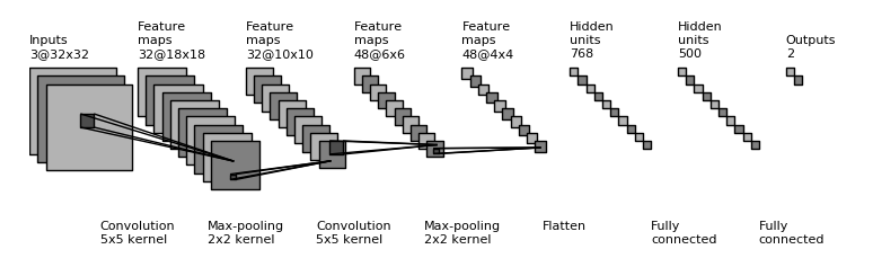
\includegraphics[width=200pt]{images/cnn/structure_CNN.png} 
\caption{Structure simplifiée d'un CNN. Source:\cite{backpropagation_cnn} }
\label{structure_1}
\end{figure}

Ainsi, l'image en entrée est d'abord traitée par une succession de \textbf{couches de convolutions} suivies d'une \textbf{couche de pooling}. Ensuite ce processus se répéte un certain nombre de fois et finalement le résultat passe par une couche dense(plus rarement plusieurs) afin de donner la bonne classification.

\subsection{Principe général}
Le principe directeur se cachant derrière les couches de convolution se base sur le fonctionnement même de notre vision : on dispose d'un noyau(pattern) capable de reconnaître un motif en particulier. Il suffit alors de balayer l'image pixel par pixel(notion expliquée plus en détails ultérieurement) pour savoir où se trouvent précisément certains motifs sur l'image. En répétant ce procédé avec un grand nombre de noyaux différents, nous sommes dans la possibilité de pouvoir identifier la présence ou non de certains motifs caractéristiques de l'objet à reconnaître. \\
Nous disposons ainsi d'une "carte" des différents motifs qu'il nous est possible de réduire en taille(étape de pooling) pour réduire le nombre de calculs à effectuer. 
Le processus se répète un certains nombre de fois jusqu'à ce que l'on considère que les données soient suffisamment bien réduites pour qu'un MLP puisse s'en charger. 

\section{Formalisation d'un CNN}

\subsection{Le produit de convolution : un outil indispensable}

Le coeur de l'efficacité d'un CNN repose sur le produit de convolution. On assimile l'image à une matrice notée $I$(nous la supposons pour l'instant en niveau de gris, de telle sorte que la matrice est en 2D mais la généralisation en 3D se fait aisément). De même, le noyau sera noté sous la forme d'une matrice $K$.
L'opération de convolution s'écrit alors : \\

$\forall (x,y) \in [|0,W_I|] \times [|0,H_I|]$,  $(N \otimes I)_{x,y} = \sum_{i=0}^{W_K} \sum_{j=0}^{H_K} K_{i,j} \times I_{x-i,y-j}$ \\
\\
Où l'on a posé $W_I,H_I$ la taille de l'image et $W_K,H_K$ la taille du noyau. \\
\\
La figure \ref{chien_prairie} donne quelques exemples de l'effet du produit de convolution avec plusieurs noyaux.

\begin{figure}[!h]
\centering
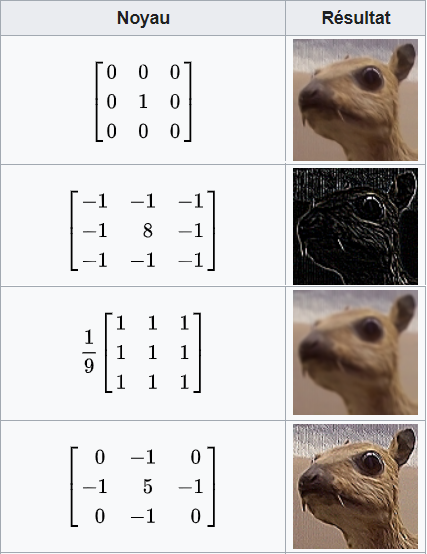
\includegraphics[width=100pt]{images/cnn/chien_prairie.png} 
\caption{Effets de la convolution avec quelques noyaux. Source: Wikipedia (c'est Paulin qui m'a dit d'écrire ça moi je voulais pas je le jure) }
\label{chien_prairie}
\end{figure}

Ainsi, cette opération nous permet de mettre en évidence des motifs élémentaires en activant la case correspondante si le motif est présent au niveau de celle-ci.

\subsection{Le balayage de l'image : une histoire de Padding et de Stride}

Pour pouvoir évaluer toute l'image, il va falloir la balayer avec le noyau. De manière assez logique, on commence par le placer sur le coin supérieur gauche de l'image, puis on affectue un produit de convolution. Ensuite, il suffit de faire glisser latéralement le noyau d'un pixel et de répéter l'opération. Une fois au bout de la ligne, on descend d'un pixel et on repart à gauche. La figure \ref{convolution} donne un exemple de balayage d'un noyau sur une image.

\begin{figure}[!h]
\centering
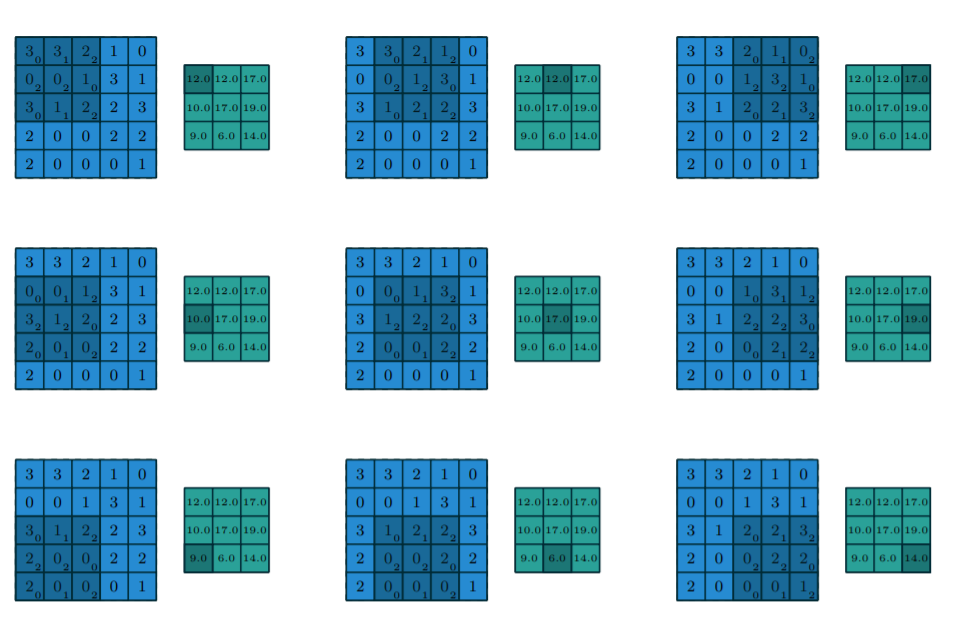
\includegraphics[width=200pt]{images/cnn/convolution.png}
\caption{Fonctionnement de la couche de convolution sur un exemple simple. Source : \cite{dumoulin_guide_2018} }
\label{convolution}
\end{figure}

On remarque alors que le résultat à une dimension plus petite que l'image d'origine : on a ici effectué ce que l'on appelle un \textbf{simple padding}. Cependant, on pourrait souhaiter que le résultat ait la même dimension : cela est rendu possible grâce au \textbf{same padding}. Pour cela, nous pouvons rajouter des gardes autour de l'image d'origine : on rajoute des zéros autour puis on effectue l'opération de convolution comme présenté sur la figure \ref{same_padding}

\begin{figure}[!h]
\centering
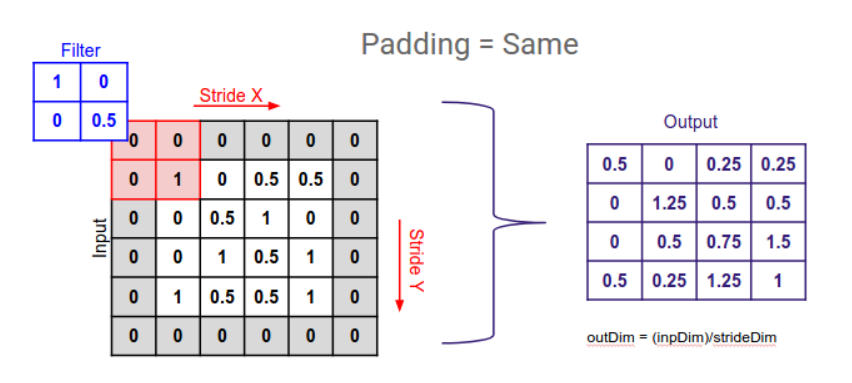
\includegraphics[width=200pt]{images/cnn/same_padding.png}
\caption{Fonctionnement de la couche de convolution avec du same padding. Source:\cite{dumoulin_guide_2018} }
\label{same_padding}
\end{figure}

Il existe encore un paramètre permettant de personnaliser l'opération : le \textbf{stride}. Celui correspond au décalage à utiliser pour le noyau. Ce processus est représenté sur la figure \ref{stride}.

\begin{figure}[!h]
\centering
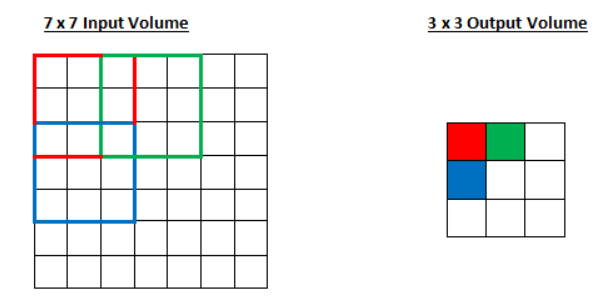
\includegraphics[width=150pt]{images/cnn/stride.png}
\caption{Fonctionnement de la couche de convolution avec un stride valant 2. A gauche le résultat de l'opération. A droite, une façon différente de voir les choses : le noyau balaye toute la matrice avec un pas de 1 mais ne garde les valeurs que pour les déplacements paires. Source:\cite{dumoulin_guide_2018}}
\label{stride}
\end{figure}
 
L'avantage d'avoir un stride plus grand que 1 est aussi son désavantage : en effet il va permettre d'avoir un résultat en sortie de plus petite dimension mais en contrepartie, il y a une perte d'information.

\subsection{Généralisation en 3D}

Les images en couleurs peuvent être représentées par une matrice 3D de profondeur 3. Pour pouvoir gérer ce cas, nous prenons des noyaux de de la même profondeur que l'image, puis nous appliquons séparément le produit de convolution sur les profondeurs correspondantes, le résultat final n'étant que la somme des résultats sur chaque profondeur. Un exemple d'une telle opération est représenté par la figure \ref{CNN_3D}.

\begin{figure}[!h]
\centering
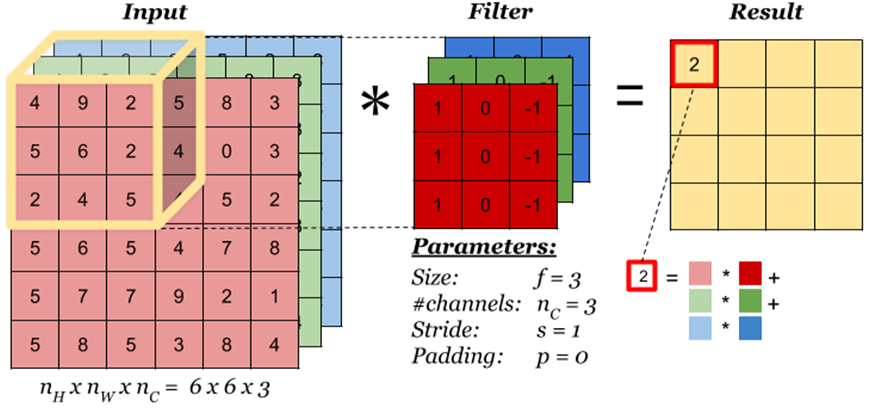
\includegraphics[width=150pt]{images/cnn/CNN_3D.png}
\caption{Exemple de convolution en 3D. Source:\cite{3D_convolution}.}
\label{CNN_3D}
\end{figure}

Notons cependant que ce résultat est très important car même si l'on considère que l'image n'a qu'une seule profondeur(image en niveau de gris par exemple), les données en entrée sur les autres couches de convolution sont dans l'immense majorité des cas en 3 dimensions. De manière intuitive, il est important de comprendre que la généralisation en 3D permet de détecter des motifs tridimensionnels au même titre qu'une opération de convolution simple permet d'identifier la présence d'un motif bidimensionnel. 

\subsection{Couche de pooling}

Les couches de pooling permettent de réduire la taille de la sortie au prix d'une perte d'information. Elles sont nécessaires dans la mesure où le nombre de calcul à effectuer sans elles rendrait le CNN  totalement inexploitable. On considère généralement deux types de couches de pooling :

\begin{itemize}
 \item max pooling : on applique un équivalent d'un noyau d'une opération de convolution qui ne retient que la valeur maximale de la zone sur laquelle il effectue les calculs. C'est la couche de pooling la plus utilisée. Un exemple de fonctionnement est présenté par la figure \ref{max_pooling}.
 
\begin{figure}[!h]
\centering
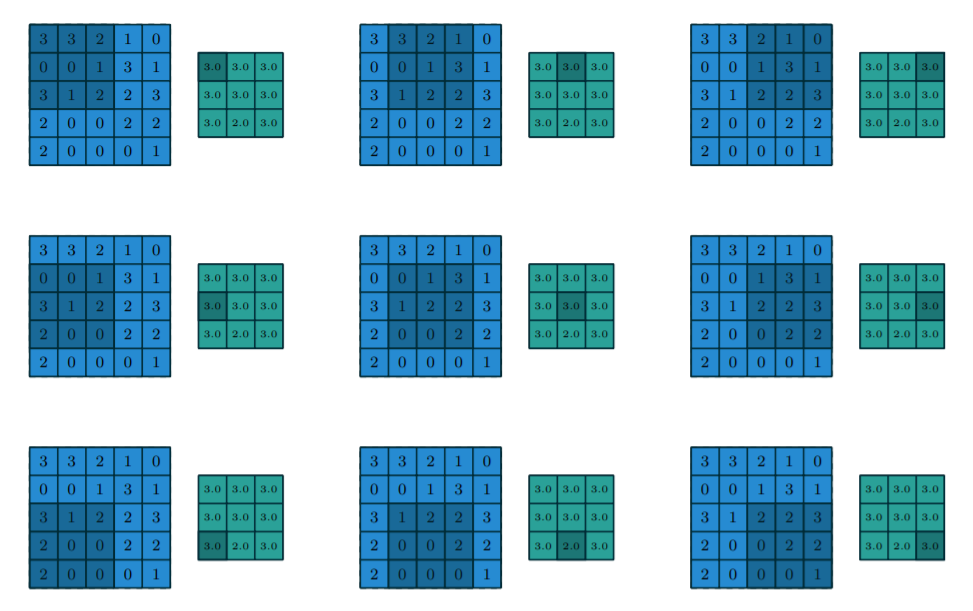
\includegraphics[width=200pt]{images/cnn/max_pooling.png}
\caption{Comparaison sur un exemple simple entre la couche de max pooling et la couche avg pooling. Source:\cite{dumoulin_guide_2018}}
\label{max_pooling}
\end{figure}
 
\item average pooling : le fonctionnement est le même que la couche de max pooling à l'exception que l'on applique la fonction moyenne au lieu de la fonction maximum. Un exemple de fonctionnement est présenté par la figure \ref{avg_pooling}.
\end{itemize}

\begin{figure}[!h]
\centering
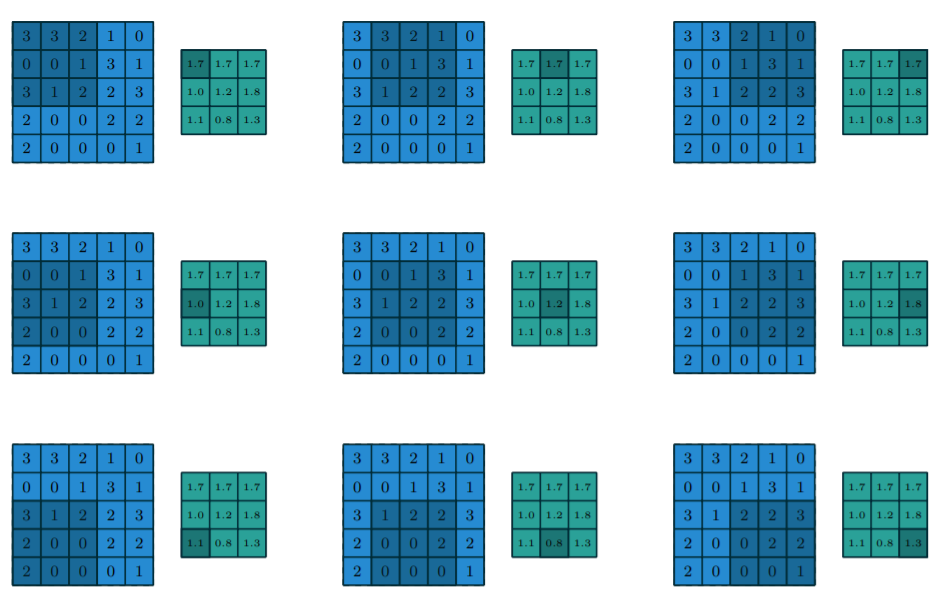
\includegraphics[width=200pt]{images/cnn/avg_pooling.png}
\caption{Comparaison sur un exemple simple entre la couche de max pooling et la couche avg pooling. Source:\cite{dumoulin_guide_2018}}
\label{avg_pooling}
\end{figure}


Il est à noter que la taille des noyaux est une variable et que plus celle-ci est grande, plus la taille de la sortie sera petite. 
\subsection{Structure complète d'un CNN}

La reconnaissance d'objet est le plus souvent complexe et nécessite de nombreux motifs à déceler pour pouvoir être efficace. Ainsi, si l'on avait un motif par couche, la taille du CNN serait gigantesque.Pour éviter cela, il suffit d'associer à chaque couche plusieurs noyaux (généralement une puissance de 2). En appliquant les processus précédant pour chacun des noyaux, on se retrouve avec un nombre de matrice en sortie égal au nombre de noyaux. On se contente alors de les empiler en rajoutant une dimension supplémentaire : on obtient alors en sortie de couche de convolution un bloc de profondeur le nombre de noyau contenant dans chacune des couches  le résultat du produit de convolution pour un noyau. La figure \ref{structure_CNN_2} illustre ce principe.

\begin{figure}[!h]
\centering
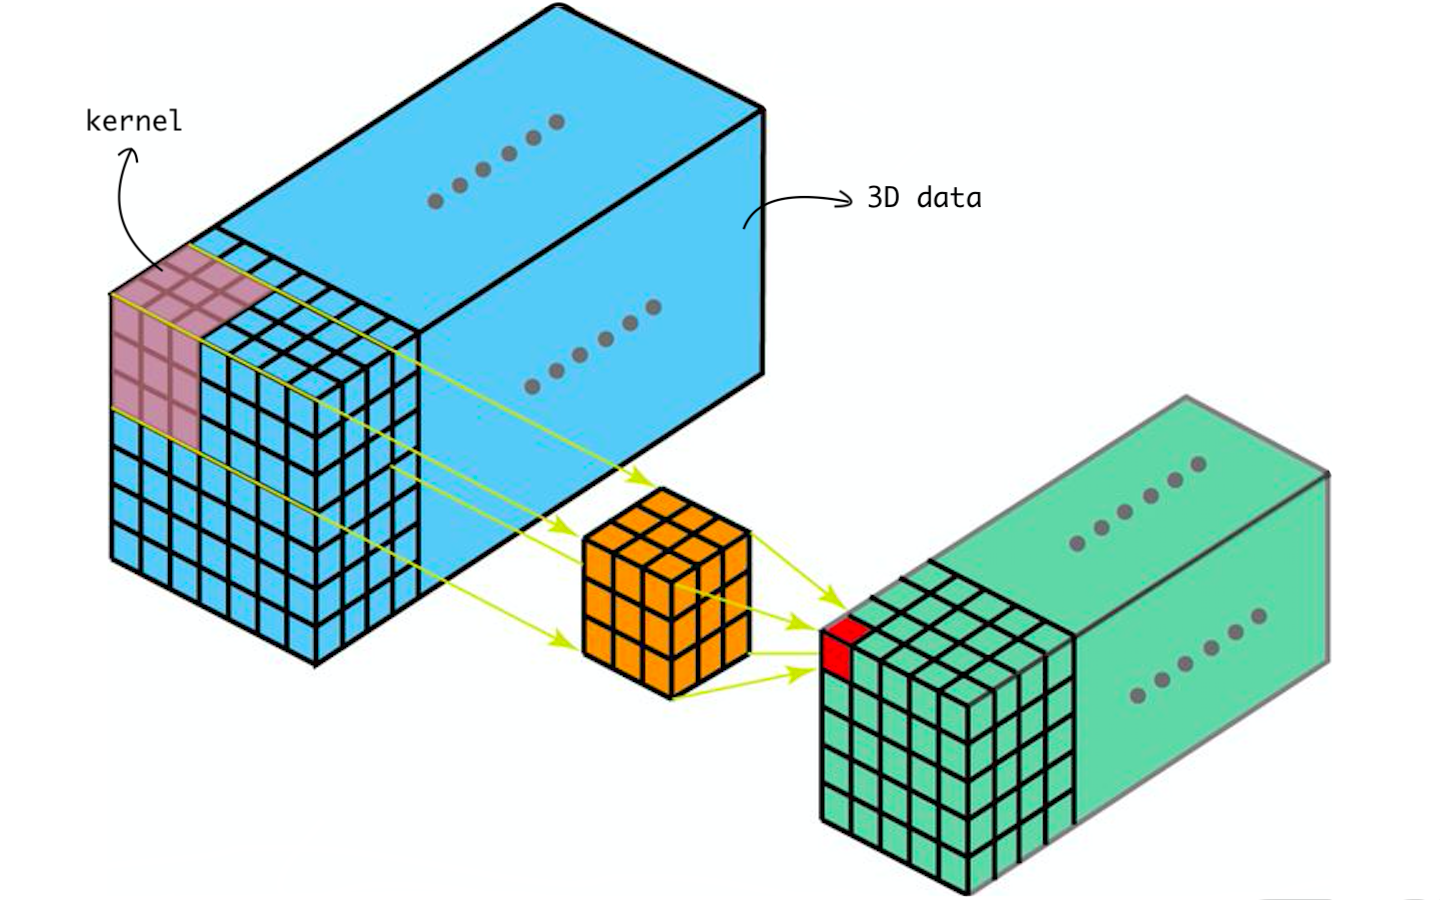
\includegraphics[width=200pt]{images/cnn/structure_CNN_2.png}
\caption{Exemple du résultat à la sortie d'une couche de convolution d'un CNN avec une structure complète. Source:\cite{3D_convolution}}
\label{structure_CNN_2}
\end{figure}

On alterne ainsi entre couches de convolution pour prélever des motifs de plus en plus complexes et couches de pooling pour réduire la quantité de calculs. Les données étant ainsi pré-traitées, il suffit de les mettre en entrée d'une couche dense pour finalement avoir le résultat escompté.

\subsection{Apprentissage d'un CNN}

Le CNN, de par sa structure analogue à celle d'un MLP, a besoin d'une phase d'apprentissage dans le but d'apprendre à reconnaitre les motifs intéressants. Cela se fait par un processus de backpropagation. Cette partie étant essentiellement calculatoire, nous ne présenterons pas les opérations exactes à effectuer dans cette section mais nous vous invitons fortement à consulter la littérature scientifique à ce sujet [ref site].

 [https://www.jefkine.com/general/2016/09/05/backpropagation-in-convolutional-neural-networks/] pour de plus amples informations.
 
\subsection{Dropout}

Le principal problème de ce type d'architecture est le phénomène de sur-apprentissage. Pour palier à ce problème, des améliorations ont été proposées, notamment en 2014 par un article[ref doc dropout] composé par des chercheurs de l'université de Toronto. Les auteurs proposent en effet d'éteindre de manière aléatoire une certaine proportion de neurones pendant la phase de forwardpropagation (cette proportion constitue un paramètre du dropout). Ils ont nommé cette technique le \textbf{dropout}. Cela permet de réduire la co-adaptation entre les neurones, évitant ainsi qu'un neurone ne prenne trop d'importance dans le processus d'apprentissage, ce qui pourrait amener à du sur-apprentissage. Une explication visuel est proposée par la figure \ref{dropout}.
 
\begin{figure}[!h]
\centering
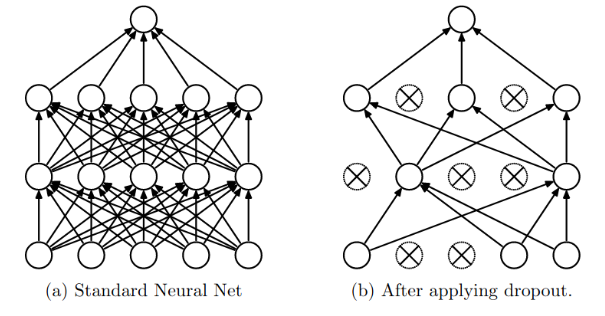
\includegraphics[width=200pt]{images/cnn/dropout.png}
\caption{A gauche : une structure MLP classique. A droite,un exemple de l'effet du dropout(paramètre ajusté à 50\%). Source : \cite{srivastava_dropout_nodate} }
\label{dropout}
\end{figure}

La figure \ref{dropout_article} présente les résultats de ce même article. Les résultats sont plus que positifs dans la mesure où la qualité prédictive du réseau est grandement amélioré par le dropout.

\begin{figure}[!h]
\centering
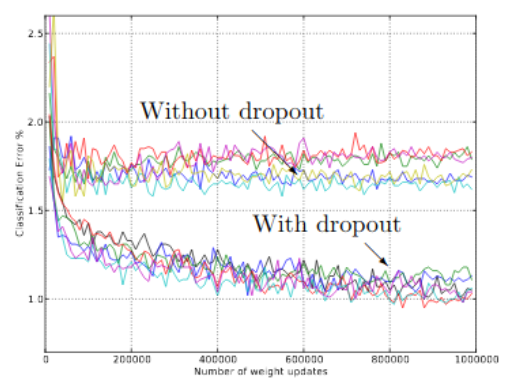
\includegraphics[width=200pt]{images/cnn/dropout_article.png}
\caption{Résultats de l'article sur l'efficacité du dropout sur un réseau neuronal. Source : \cite{srivastava_dropout_nodate} }
\label{dropout_article}
\end{figure}
 
\section{Implémentation et résultats}

\subsection{Implémentation}

Nous avons une nouvelle fois utilisé TensorFlow 2.0 qui permet l'utilisation rapide de couches telles que celles de convolution, de pooling mais aussi de flatenning : c'est une couche permettant de faire la transition entre la dernière couche de convolution et la première couche dense. En d'autres termes, elle transforme les données en 3 dimensions en un tableau en 1 dimension.

\[ \begin{array}{lcr}
	Conv2D(64, 3, activation='relu') \\
    Conv2D(32, 3, activation='relu') \\
    Flatten() \\
    Dense(128, activation='relu') \\
    Dense(10, activation='softmax')\end{array}\]

Nous avons de plus utilisé l'optimiseur ADAM pour effectuer la descente de gradient.

\subsection{Résultats}

Nous avons tout d'abord voulu tester la taille des noyaux pour voir quelle influence celle-ci a sur les performances de notre CNN. La figure \ref{resultat_noyaux} présente les résultats sur la base de données MNIST.

\begin{figure}[!h]
\centering
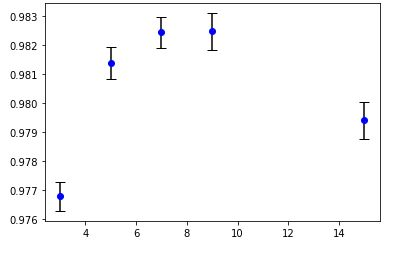
\includegraphics[width=100pt]{images/cnn/resultat_noyau.png}
\caption{Comparaison de l'efficacité de notre CNN en fonction de la taille des noyaux. La base de données utilisée est MNIST.}
\label{resultat_padding_stride}
\end{figure}

Nous pouvons en déduire que des noyaux de taille trop grande par rapport aux images d'origine risquent de nuire à l'efficacité du CNN. \\

Nous nous sommes de plus intéressé à l'influence du \textbf{stride} et du \textbf{padding} sur les performances du CNN. La figure \ref{resultat_padding_stride} présente les résultats de notre analyse sur MNIST.

\begin{figure}[!h]
\centering
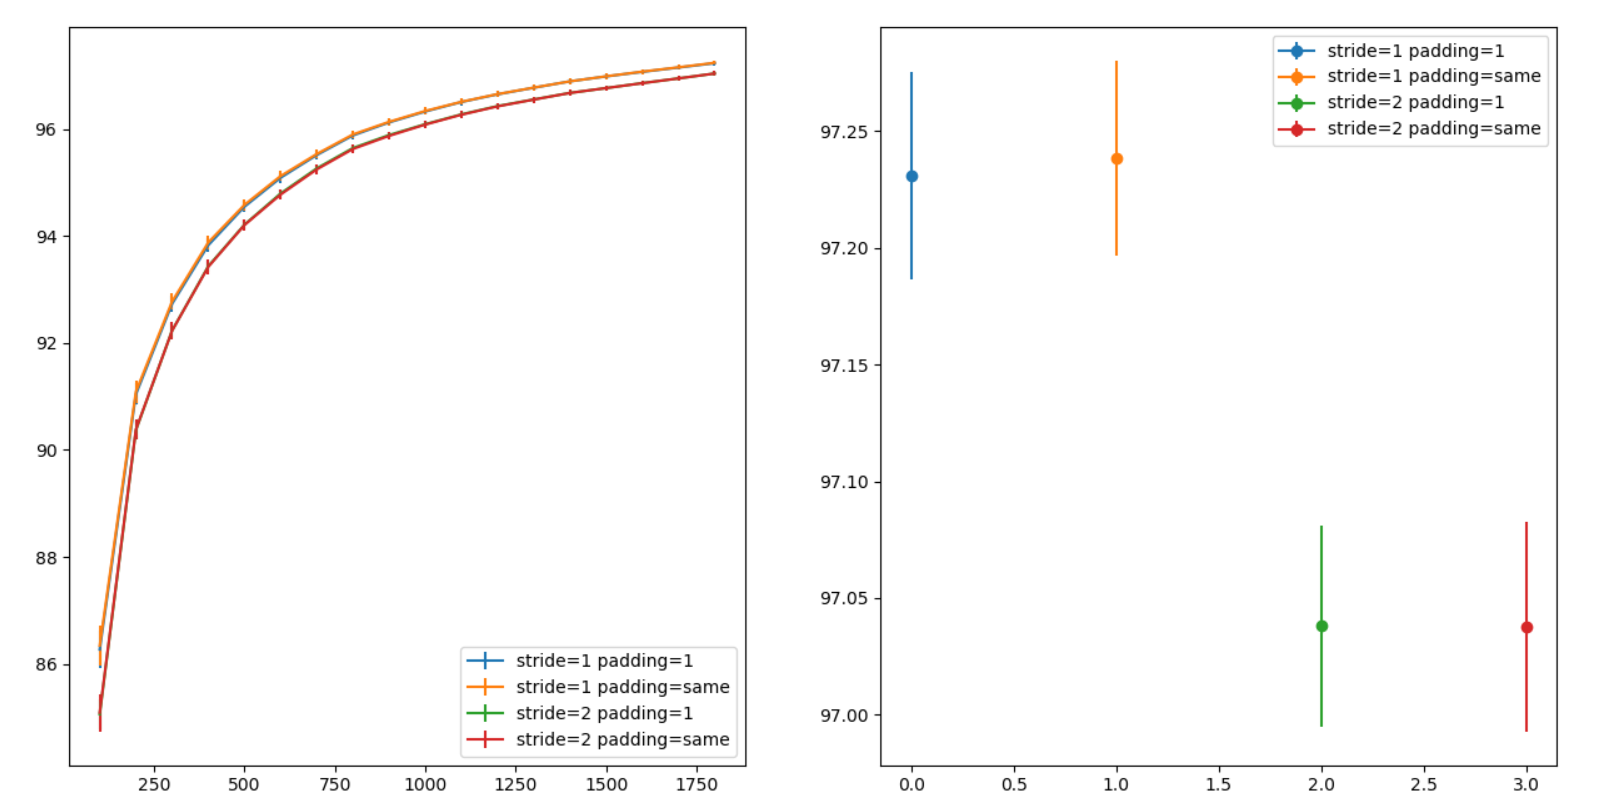
\includegraphics[width=200pt]{images/cnn/CNN_padding_stride.png}
\caption{Comparaison de l'efficacité de notre CNN en fonction des paramètres stride et padding. La base de données utilisée est MNIST.}
\label{resultat_padding_stride}
\end{figure}

Nous pouvons conclure que sur cette base de données, l'utilisation d'un stride supérieur à 1 a comme effet de réduire les capacités prédictives du CNN. En effet, lorsque ce paramètre est trop élevé, la perte d'information est trop importante, nuisant aux performance de l'algorithme. Nous remarquons de plus que le padding n'a ici aucune influence. Cependant, ce résultat est à prendre avec prudence car les images de MNIST sont centrées avec des bords sombres.Ainsi il n'y a aucunes informations sur les bords, rendant le changement de padding quasiment inutile. \\

De même, nous avons testé l'influence du \textbf{dropout}. Les résultats sont présentés sur la figure \ref{resultat_dropout}.
  
\begin{figure}[!h]
\centering
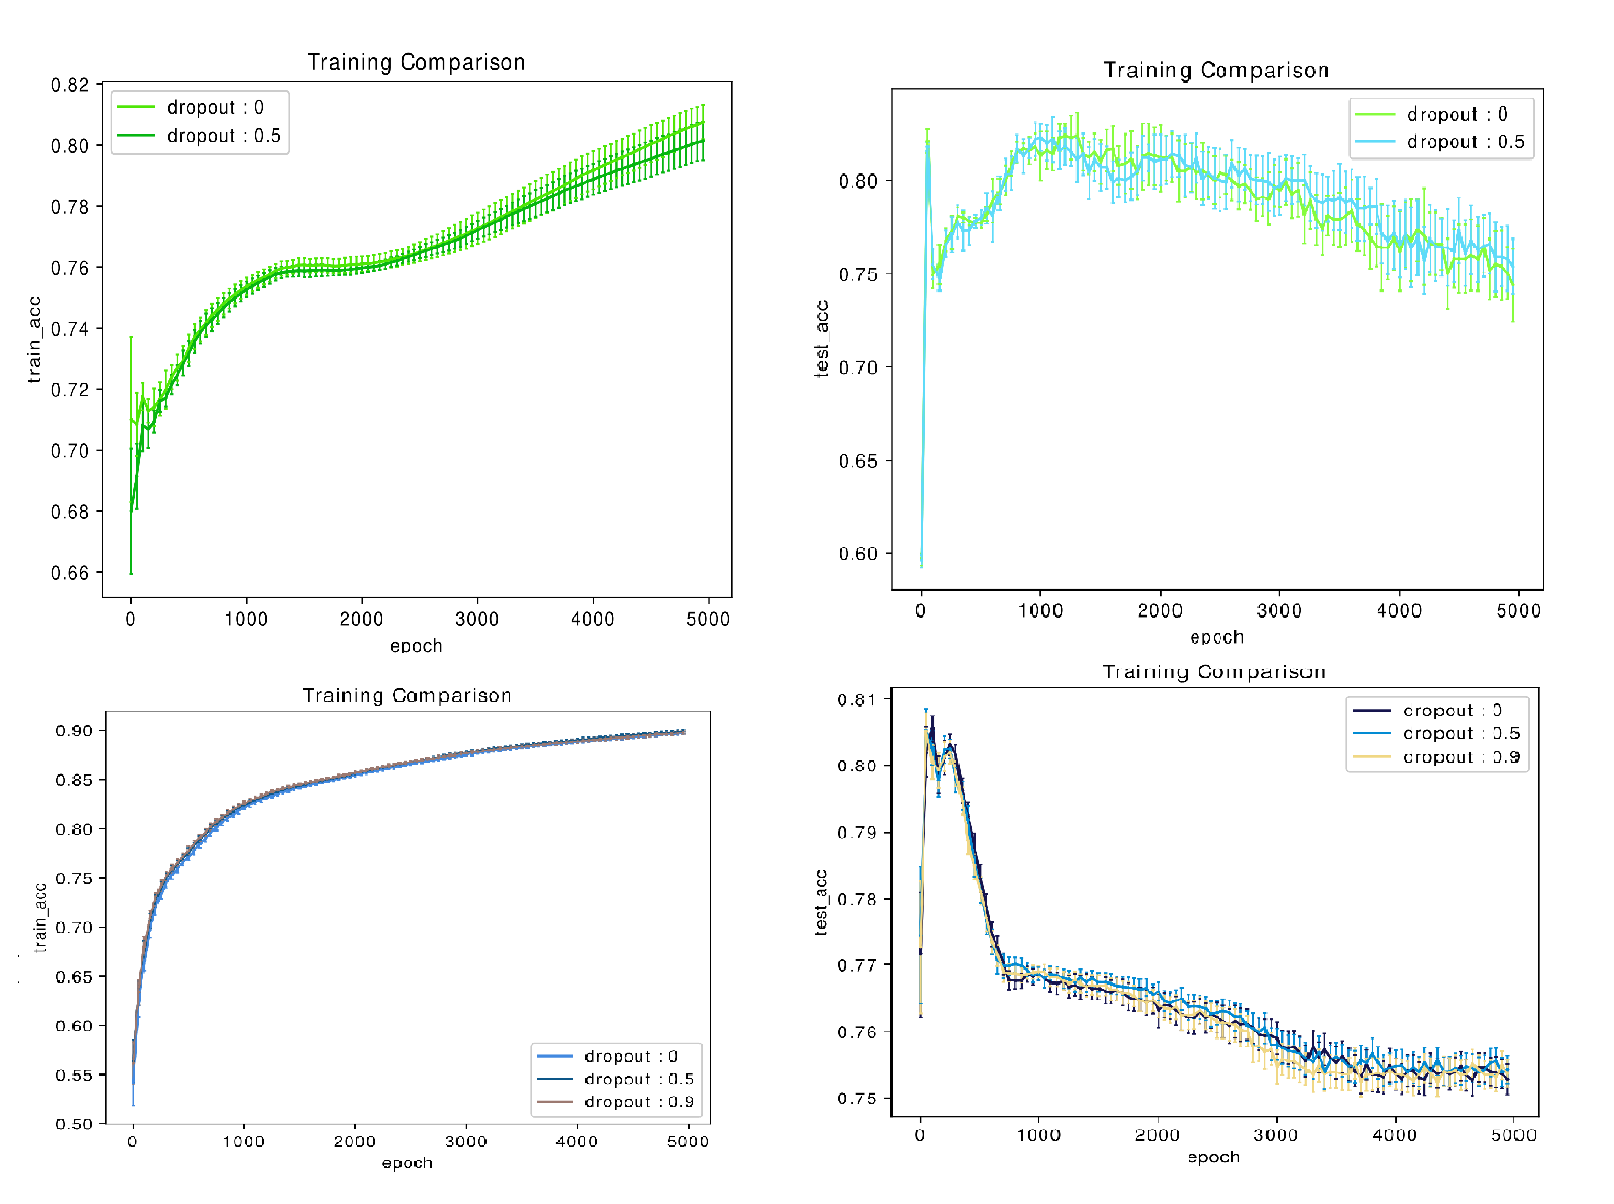
\includegraphics[width=200pt]{images/cnn/resultat_dropout.png}
\caption{Influence du dropout sur l'efficacité de nos réseaux. En haut, un CNN sur la base de données MNIST.En bas, un MLP sur la base de données Moon. Nous remarquons que les courbes sont toutes confondues, quelque soit le paramètre de dropout choisi.}
\label{resultat_dropout}
\end{figure}

Les résultats sont beaucoup moins significatifs que ce que laisse présager l'article [ref]. Il semble donc que le dropout n'ai aucune influence sur les résultats de notre CNN. 

https://www.cs.princeton.edu/courses/archive/spr08/cos598B/Readings/Fukushima1980.pdf




\chapter{Les GAN (Réseaux Adverses Génératifs)}

\section{Principe général des GAN}
Le principe général des GAN repose sur l'utilisation de deux réseaux, ayant des objectifs contraires, on dit qu'ils sont \textbf{adversaires}. Le premier réseau transforme du bruit en image, c'est le \textbf{générateur} (G). Le deuxième réseau prend en entrées des images et les classe en deux catégories en leur associant leur probabilité d'être issues de la base de donnée. C'est donc un classifieur binaire, il est appelé \textbf{discriminateur} (D). Le plus souvent, le discriminateur sera alimenté par des images de deux sortes : celles provenant de la base de donnée (images réelles), et celles générées par le générateur, son rôle sera donc de dire si une image est réelle ou générée. Il s'agit ensuite d'entraîner G afin qu'il maximise la probabilité que D fasse une erreur, et d'optimiser D afin qu'il améliore la justesse de sa classification.

L'architecture des GAN a été introduite pour la première fois par Ian Goodfellow \cite{goodfellow_generative_2014} en 2014. Cet article innovant montrait déjà un gain de performance pour la génération d'images suivant une base de donnée. Mais l'atout majeur des GAN sont leur adaptabilité à tous types de données.


\section{Le DCGAN (Deep Convolutionnal Adversarial Network)}
Le DCGAN utilise la fonction de coût proposée par Goodfellow \cite{goodfellow_generative_2014}, mais le générateur et le discriminateur sont tous les deux des \textbf{réseaux à convolutions} \cite{radford_unsupervised_2015-1}. La fonction de coût de G à minimiser est la suivante : $$\begin{aligned}
\mathcal{L}_{\mathrm{DCGAN}}\left(G, D, p_{\mathrm{data}}, p_{\mathrm{bruit}}\right) &=
   \mathbb{E}_{x \sim p_{\mathrm{data}}}(\log (D(x))) + \mathbb{E}_{z \sim \mathrm{p_{bruit}}}(\log (1 - D(G(z)))
\end{aligned}$$

Pareillement, on donne comme fonction de coût pour D l'opposé de celle de G. L'architecture du DCGAN correspond alors à un jeu à somme nulle. La théorie des équilibres de Nash donne un unique état stable. Il correspond à un coût égal à $-\log 4$ pour G et $ \log 4$ pour D. Dans cette configuration, le discriminateur est forcé d'associer une probabilité de 0,5 pour chaque image donnée en entrée, le générateur étant devenu trop fort.

Une variation intéressante sur le DCGAN est de poser $  \mathbb{E}_{x \sim p_{\mathrm{data}}}(\log (D(x))) + \mathbb{E}_{z \sim \mathrm{bruit}}(\log (D(G(z)))$ comme fonction de coût en début d'apprentissage. L'intérêt de cette modification résulte d'un problème : le discriminateur a tendance à facilement distinguer les images générées par G de celles de la base de donnée en début d'apprentissage. Dans ce cas, le terme $\log (1 - D(G(z))$ sature vers 0. Le remplacer par $\log (1 - D(G(z))$ résout ce problème.


\section{Étude de la convergence des GAN}

De par leur caractère d'adversaires, les GAN requièrent un équilibre fin entre la générateur et le discriminateur, ils sont donc par nature \textbf{instables}. L'étude de la convergence des GAN est un domaine encore très actif de la recherche. Nous allons discuter de deux phénomènes très communs qui peuvent gêner ou ruiner l'apprentissage des GAN : l'\textbf{effondrement des modes} (\textit{mode collapse}), et la \textbf{non-convergence} due à la perte d'équilibre du système.

\subsection{L'effondrement des modes}

\begin{figure}[!h]
\centering
\includegraphics[width=100pt]{"images/GAN/collapseA_1"}
\includegraphics[width=100pt]{"images/GAN/collapseA_2"}
\caption{Exemples d’effondrement des modes sur la banque de chiffres MNIST.}
\label{mode_collapse}
\includegraphics[width=100pt]{"images/GAN/collapseB_1"}
\includegraphics[width=100pt]{"images/GAN/collapseB_2"}
\caption{À gauche, un exemple d'effondrement des modes sur la banque d'image CelebA. À droite, une génération sans effondrement pour comparaison. On observe que sur l'image de gauche, tous les personnages ont la même tête.}
\label{mode_collapse_celeb}
\end{figure}


L'effondrement des modes survient quand le réseau générateur ne génère pas des images conforment à l'ensemble de la distribution des images réelles, mais seulement à une petite partie. L'effondrement des modes est très visible lorsque la distribution des images réelles forme des zones bien séparées, c'est à dire quand celle-ci comporte des classes bien définies. La manifestation de ce phénomène se traduit par des images générées qui se ressemblent toutes. Les figures \ref{mode_collapse} et \ref{mode_collapse_celeb} montrent des exemples du phénomène sur la base de données MNIST et CelebA.


Pour mieux comprendre le phénomène, il est intéressant de regarder la distribution des images de MNIST dans son ensemble. Cela est possible grâce à des algorithmes de réduction de dimension. Attention, la réduction de dimension se fait dans l'espace des pixels, et non pas dans un espace sémantique. La visualisation ne permet donc pas de séparer efficacement les différentes classes, elle permet seulement un aperçu de la distribution des images de la banque. Les figures \ref{tsne1} et \ref{tsne2} présentent une visualisation de MNIST par transformation t-SNE \cite{van_der_maaten_visualizing_2008}.

\begin{figure}[!h]
\centering
\includegraphics[height=90pt]{"images/GAN/modes1"}
\includegraphics[height=90pt]{"images/GAN/modes1_tsne"}
\caption{On observe un effondrement à deux modes. Le GAN ne génère que des chiffres 1 et des chiffres 8, correspondant aux point rouges sur la représentation t-SNE.}
\label{tsne1}
\includegraphics[height=90pt]{"images/GAN/modes2"}
\includegraphics[height=90pt]{"images/GAN/modes2_tsne"}
\caption{On observe un effondrement à un mode, donc tous les points rouges sont regroupés. De plus le GAN génère un symbole non présent dans la base MNIST, donc les points rouges ne correspondent à aucun nuage de points de la banque d'images.}
\label{tsne2}
\end{figure}

L'ensemble de points rouges correspond à un ensemble d'images générées par le réseau générateur lors de l'effondrement des modes. Sur les données MNIST, on observe différents groupes de points (des \textit{clusters}), ce sont les \textbf{modes} inhérents à la base de donnée MNIST : les chiffres de 1 à 9. Ce qu'il est intéressant de noter, c'est que les points générés sont rassemblés autour de un ou plusieurs pôles denses très localisés, qui ne sont pas répartis dans tout l'espace. Cela traduit l'effondrement des modes : les images générées ne couvrent qu'une petite partie de la distribution de la base de donnée d’entraînement.\\

Il n'y a pas de solution simple, directe et universelle pour lutter contre l'effondrement des modes, mais quelques solutions ont été proposées :
\begin{itemize}
  \item La pénalisation de la similarité des images en sortie de générateur, c'est la \textit{minibatch discrimination}. Cela consiste à ajouter un terme à la fonction de coût pour traduire la similarité (il peut s'agir de calculer une similarité pixel à pixel, ou d'estimer la similarité sémantique grâce un autre réseau de neurones).
  \item Le \textit{one-side label smoothing}. Cela consiste à changer l'objectif du discriminateur : son objectif ne sera plus de discriminer les fausses images avec une probabilité de 1, mais une probabilité plus faible, par exemple 0.9. Cela permet d'éviter la sur-confiance, et permet de laisser le générateur explorer tous l'espace des images réelles.
  \item Certaines architectures sont plus résistantes que d'autres à l'effondrement des modes. Par exemple, les GAN de Wasserstein [\ref{WGAN}] ne présentent ce problème. 
\end{itemize}


\subsection{Perte de l'équilibre}

Comme expliqué plus haut, l'apprentissage des GAN repose sur un équilibre fin entre le discriminateur et le générateur. Cet équilibre est parfois difficile à atteindre et est souvent instable, c'est pourquoi parfois le système s'effondre complètement. Cet effondrement vient souvent du fait que le discriminateur est devenu "trop fort" (sa fonction de perte tombe à zéro), et le générateur ne peut plus s'améliorer. Lorsque cela arrive, l’entraînement peut être arrêté : les images générées ne s'amélioreront plus. Un exemple de ce phénomène et illustré dans la figure \ref{perte_eq}, où l'on voit qu'à partir d'un cycle d’entraînement, la fonction de perte du discriminateur s'écroule et celle du générateur diverge.

\begin{figure}[!h]
\centering
\includegraphics[width=100pt]{"images/GAN/failure1"}
\includegraphics[width=100pt]{"images/GAN/failure2"}
\includegraphics[width=100pt]{"images/GAN/failure3"}
\caption{}
\label{perte_eq}
\end{figure}


Il existe des solutions pour lutter contre ce problème, et cela consiste souvent à rééquilibrer les puissances ou les vitesses de convergence des différents réseaux. On peut par exemple diminuer la complexité du discriminateur, diminuer le taux d'apprentissage du discriminateur, ou mettre à jouer plus souvent le générateur que le discriminateur.
Ajouter du bruit sur les images de la base de donnée permet aussi se renforcer la stabilité de l'apprentissage. Par ailleurs, on peut noter que les GAN de Wassertein sont plus stables que les DCGAN, mais ne sont pas totalement immunisés aux problèmes de convergence.

\section{Cadre théorique et WGAN}
Nous allons essayer dans cette section de donner un cadre probabiliste et statistique rigoureux permettant d'expliquer le fonctionnement des GAN. Cette approche permettra de justifier l'algorithme WGAN qui permet de significativement réduire les problèmes d'apprentissage des GAN.

\subsection{Approche bayésienne des GAN}
L'objectif d'un GAN - la génération d'images suivant un dataset - peut être formalisé comme un problème d'optimisation bayésienne. Nous cherchons à approcher la distribution $p_{\mathrm{data}}$ d'une variable aléatoire $X: \Omega \longrightarrow \mathcal{X}$. Pour ce faire, on se donne une famille paramétrique de distributions $\mathcal{M}_{\mathbb{R}^{d}} = \{p_{\theta}, \theta \in \mathbb{R}^d\}$, ainsi qu'un prior $p_{\mathrm{bruit}}(z)$ relatif à une variable aléatoie $Z : \Omega \longrightarrow \mathcal{Z}$. On détermine ensuite la distribution souhaitée à l'aide de la formule de Bayes. $$\begin{aligned} p(\theta | \mathrm{data}) \propto p_{\mathrm{bruit}}(z)p(\mathrm{data}|\theta)\end{aligned}$$

Comme il est impossible de résoudre directement la formule de Bayes, il nous faut défnir une fonction de côut qui mesure la distance entre $p_{\theta}$ et $p_{\mathrm{data}}$, puis employer des algorithmes de descente du gradient. La famille $\mathcal{M}_{\mathbb{R}^d}$ prend alors naturellement la forme d'un réseau de neurones, que l'on écrit $g : \mathcal{Z} \times \mathbb{R}^{d} \longrightarrow \mathcal{X}$, ou en notation condensée $g_{\theta}(z)$ .

\subsection{DCGAN} \label{DCGAN_prob}

Le DCGAN utilise la métrique $\delta$ pour mesurer l'écart entre deux distributions $p_{\mathrm data}$ et $p_{\theta}$, définie par la relation suivante. 

$$\begin{aligned} \delta(p_{\mathrm{data}}, p_{\theta}) = -\log 4 + 2 \mathrm{DJS}(p_{\mathrm{data}} || p_{\theta})\end{aligned}$$ où DJS est la divergence de Jensen-Shanon.

On peut montrer \cite{goodfellow_generative_2014} la relation suivante, en posant $\mathcal{F}$ l'ensemble des fonctions continues $\mathcal{X} \longrightarrow (0,1)$.

$$\begin{aligned} \delta(p_{\mathrm{data}}, p_{\theta}) = \sup_{f\in\mathcal{F}} \mathbb{E}_{x \sim p_{\mathrm{data}}}(\log (f(x))) + \mathbb{E}_{x \sim p_{\theta}}(\log (1 - f(x)))\end{aligned}$$

On remarque alors si $f: \mathcal{X} \longrightarrow (0,1)$ est solution de ce problème on peut calculer $\nabla_{\theta} \delta$, dans l'optique d'optimiser $g_{\theta}(z)$. 

$$\begin{aligned}\nabla_{\theta} \delta(p_{\mathrm{data}}, p_{\theta}) = \mathbb{E}_{z\sim p_{\mathrm{bruit}}(z)} \left( \frac{\nabla_{\theta}f(g_{\theta}(z))}{f(g_{\theta}(z)) -1} \right)\end{aligned}$$.

Il nous reste encore à déterminer $f$. Il est intuitif de chercher à calculer $f$ comme un réseau de neurones $\{f_{w}, w \in \mathcal{W} \}$, qui peut être optimisé par rétropropagation à partir de  $\mathbb{E}_{x \sim p_{\mathrm{data}}}\left(\frac{\nabla_{w}f_{w}(x)}{f_{w}(x)}\right)+ \mathbb{E}_{z \sim p_{\mathrm{bruit}}}\left(\frac{\nabla_{\theta}f(g_{\theta}(z))}{f(g_{\theta}(z)) -1}\right)$.

Ce formalisme nous renvoie donc à la définition du DCGAN par sa fonction de coût pour G (ici $g_{\theta}$) et D (ici $f_{w}$). En effet, on a la relation suivante : 

$$\begin{aligned}
\delta(p_{\mathrm{data}}, p_{\theta}) = \sup_{f\in\mathcal{F}} \mathcal{L}_{\mathrm{DCGAN}}(g_{\theta}, f, p_{\mathrm{data}},  p_{\mathrm{bruit}})
\end{aligned}$$

\subsection{WGAN} \label{WGAN}

Les Wasserstein GAN, ou WGAN, on été introduits en 2017 par Arjovsky et al. \cite{arjovsky_wasserstein_2017}. Les auteurs y introduise une nouvelle distance, la distance 1-Wasserstein (qu'on appelera ici distance Wassertein), définie par la relation suivante:

$$\begin{aligned}
W(p_{\mathrm{data}}, p_{\theta}) = \inf_{\gamma \in \Pi (p_{\mathrm{data}}, p_{\theta})} \mathbb{E}_{(x, y) \sim \gamma} (||x - y||)
\end{aligned}$$
Avec $\Pi (p_{\mathrm{data}}, p_{\theta})$ l'ensemble des densité de distributions jointes $\gamma (x, y)$ de lois marginales respectivement $p_{\mathrm{data}}$ et $p_{\theta}$. On peut réecrire ce résultat à l'aide de la formulation duale du théorème de Kantorovich \cite{villani_optimal_2006}.


$$\begin{aligned}
W(p_{\mathrm{data}}, p_{\theta}) = \sup_{f \in L_{1}}\left(\mathbb{E}_{x\sim p_{\mathrm{data}}} [f(x)] - \mathbb{E}_{x\sim p_{\theta}} [f(x)]\right)
\end{aligned}$$
 Avec $L_{1}$ l'ensemble des fonctions 1-lipschitziennes $\mathcal{X} \longrightarrow \mathbb{R}$. On obtient donc une équation assez similaire à celle du paragraphe \ref{DCGAN_prob}. Nous allons estimer $f$ par un réseau de neurones $\{f_{w}, w \in \mathcal{W} \}$ qui sera optimisé à l'aide du gradient $\mathbb{E}_{x\sim p_{\mathrm{data}}} \left[\nabla_{w}f_{w}(x)\right] - \mathbb{E}_{z\sim p_{\mathrm{bruit}}} \left[\nabla_{w}f_{w}(g_{\theta}(z))\right]$. De même, à $f$ fixé, $g_{\theta}(z)$ s'optimise par rétropagation du gradient selon $\theta$.
 
 \subsection{Avantages comparatif du WGAN par rapport au DCGAN}
 
Maintenant que nous savons ce qu'est un WGAN, il s'agit de comprendre son avantage par rapport au DCGAN. D'abord, la distance $W$ est topologiquement plus faible que la divergence de Jensen-Shanon, et donc par extension que $\delta$. Ceci signifie qu'il est plus facile en pratique de faire converger un WGAN qu'un DCGAN.

Ensuite, à chaque boucle d'apprentissage, le WGAN peut mieux optimiser le discriminateur avant de faire apprendre le générateur. En effet, pour un WGAN, meilleur est le discriminateur, meilleur est le gradient utilisé pour l'apprentissage du générateur. Ceci permet de résoudre le problème d'instabilité au début de l'apprentissage rencontré dans les DCGAN, pour lesquels un discriminateur trop bon fait saturer le gradient du générateur à 0.

Finalement, la capacité du WGAN d'entraîner d'abord le discrimnateur empêche le phénomène du mode collapse. En effet, la cause du mode collapse est que pour un discriminateur fixé, le meilleur générateur est celui qui ne génère que les points de $\mathcal{X}$ de plus grande valeur pour le discriminateur.

\section{Implémentation et résultats}

Nous avons implémenté avec succès l'algorithme WGAN pour la base de donnée MNIST, et  DCGAN pour les banques de données MNIST et CelebA. 

\subsection{Détails de l'implémentation}

Nous avons utilisé la même structure de réseau pour le DCGAN et le WGAN, en changeant uniquement la fonction de coût.


\textbf{Pour le discriminateur :},
\[ \begin{array}{lcr}
Conv2D(64, (5,5), strides=(2,2)) \\
LeakyReLU() \\
Dropout\\

Conv2D(128, (5,5), strides=(2,2)) \\
BatchNormalization\\
LeakyReLU()\\
Dropout\\

Conv2D(256, (5,5), strides=(2,2)) \\
BatchNormalization\\
LeakyReLU()\\
Dropout\\


Flatten()\\
Dense(1)\\
LeakyReLU()\\

\end{array}\]

\textbf{Pour le générateur :} 

\[ \begin{array}{lcr}
Dense(240)\\
LeakyRelu()\\
Reshape((10, 8, 3))\\

Conv2DTranspose(256, (5,5), strides=(2,2)) \\
BatchNormalization\\
LeakyReLU() \\


Conv2DTranspose(64, (5,5), strides=(2,2)) \\
BatchNormalization\\
LeakyReLU() \\

Conv2DTranspose(3, (5,5), strides=(2,2)) \\

\end{array}\]

\subsection{MNIST}

Nous présentons ici les résultats obtenus après 50 passes sur la base de données MNIST, à l'aide des algorihtmes DCGAN et WGAN. On observe que nous avons eu plus de mal dans l'implémentation du WGAN, et n'arrivons pas à obtenir le gain de performance prédit par l'article \cite{arjovsky_wasserstein_2017}.

\begin{figure}[!h]
\centering
\includegraphics[width=100pt]{"images/GAN/MNIST_DCGAN"}
\includegraphics[width=100pt]{"images/GAN/MNIST_WGAN"}
\caption{A gauche, 16 images générées par le DCGAN. A droite, 16 images générées par le WGAN}
\label{mnist_gan}
\end{figure}

\subsection{CelebA}

Nous présentons ici les résultats obtenus après 400 passes sur la base de données CelebA. Nous avons donc réussi à construire avec succès un générateur de visages réalistes sans mode collapse.

\begin{figure}[!h]
\centering
\includegraphics[width=300pt]{"images/GAN/DCGAN"}
\caption{39 images obtenues par DCGAN sur la base CelebA}
\label{celeb_gan}
\end{figure}
\chapter{Le cycleGAN}

\section{Présentation de la problématique}

[AJOUTER DES REFS]

Les cycleGAN sont des architectures de GAN qui permettent de répondre à une problématique bien spécifique : le \textbf{transfert de style non appairé}, que nous expliciterons.

Le transfert de style consiste à transformer des données d'un \textit{style à un autre}. Le terme de \textit{style} est à prendre au sens large et les données que l'on manipule peuvent être de natures diverses. Il peut s'agir par exemple de transformer des images de pommes en images d'orange, de transformer un paysage d'été en un paysage d'hiver, de transformer une musique classique en rock, ou encore de modifier l'expression les expressions faciales d'individus présents sur une image. Le cycleGAN peut aussi résoudre des problèmes de segmentation d'images, en considérant la segmentation comme un style pour l'image. Quelques exemples sont présentés sur la figure ??.

\begin{figure}[!h]
\centering
\includegraphics[width=150pt,valign=t]{"images/cycle_exemples"}
\caption{legende}
\end{figure}


Le transfert de style peut s'effectuer entre plusieurs \textit{classes de styles}, mais nous allons ici nous concentrer dans le cas binaire où l'on considère deux styles. La problématique est donc de transformer des images d'un style à l'autre, et ceci dans les deux sens.

Le transfert de style (à deux classes), repose sur deux banques de données, que l'on notera A et B. Suivant les données auxquelles nous avons accès, il existe deux cas différents :
\begin{itemize}
  \item Dans le cas où nous connaissons un appairage entre les images de A et de B, le problème est un \textbf{transfert de style appairé}. Le but est donc d'apprendre et de généraliser le transfert d'une donnée de A à une donnée de B à partir d'exemples de paires déjà existantes.\\
  \textit{Par exemple, si A représente des bâtiments de jour, et B représente des bâtiments de nuit, il est possible de prendre la même photo de jour et de nuit. Ces deux photos constituent une paire dont chaque élément est d'un style différent.}.
  \item Dans le cas où chaque élément de A n'a pas de lien direct avec un élément de B en particulier, le problème est un \textbf{transfert de style non appairé}. Le but n'est plus d'apprendre et de généraliser le transfert d'une donnée de A à une donnée de B à partir d'exemples de paires déjà existantes, mais d'apprendre le transfert entre le style de A et le style de B, sans avoir d'exemple d'une telle transformation. Il faut donc \textit{comprendre} à un niveau sémantique les style de A et B.\\
  \textit{Par exemple, si vous voulez transformer une image de votre chien en image de chat, vous ne pouvez pas obtenir une banque d'image de chiens déguisés en chats. Vous devez donc travailler avec d'une part des images de chiens (A), d'autre part des images de chats (B), sans pouvoir former de paires entre A et B.}\\
   La différence entre ces deux cas est illustrée par la figure ??. 
\end{itemize}

\begin{figure}[!h]
\centering
\includegraphics[width=100pt,valign=t]{"images/paire"}
\hspace*{10mm}
\includegraphics[width=100pt,valign=t]{"images/pairepas"}
\caption{legende (pas beau !!}
\end{figure}

Ces deux types de transfert de style se traitent différemment. Pour le transfert de style appairé, une structure de GAN classique suffit puisque le discriminateur peut aisément comparer l'image générée avec l'image \textit{idéale}. Ce problème, que nous ne développerons pas ici, est traité et manière efficace par différents algorithmes, dont \textbf{Pix2Pix}. Le transfert de style non appairé ne permet pas la comparaison à l'image-cible puisqu'il n'existe pas de paires. \textbf{Il faut donc utiliser d'autres architectures, comme par exemple le cycleGAN.}


\section{Principe général du cycleGAN}

En vertu des explications présentées au paragraphes précédent, le problème se présente ainsi : nous avons une banque de données structurées A, et une banque de données structurées B, de même nature, dont les styles sont différents. Dans la suite, nous nous placerons dans le cas où s'est données sont des images. Le but est de transformer les images de A pour leur donner le style des images de B, et inversement.

Le cycleGAN repose sur deux GAN, tête-bêche, l'un permettant de passer du style A au style B, l'autre du style B au style A. Plus précisément, il y a deux générateurs, un générateur qui prend des images de la banque A et doit générer des images du style de B (noté G), l'autre qui prend des images de la banque B et doit générer des images du style de A (noté F). Il y a aussi deux discriminateurs, notés $D_A$ et $D_B$, qui respectivement discriminent des images du style A et celles du style B. L'architecture est présenté par la figure ??.

\begin{figure}[!h]
\centering
\includegraphics[width=200pt]{"images/cycleDouble"}
\caption{legende (figure à changer)}
\end{figure}

Comme on l'a entrevu dans le paragraphe précédent, une difficulté est que les données ne sont pas appairées, la fonction de coût ne peut donc pas venir de la comparaison directe de l'image générée à l'image souhaitée. Pour pallier à ce manque, deux fonctions de coûts principales et indépendantes sont utilisées.\\

La première est celle d'un GAN classique : pour une transformation $ A \rightarrow B $ (resp. $ B \rightarrow A $), le discriminateur $ D_B $ (resp. $ D_A $) prédit si l'image est une image qui appartient réellement à la banque B (resp. A). Le coût associé au GAN ainsi défini est appelé \textit{Adversarial Loss} ou \textit{GAN Loss}. La figure ?? montre la décomposition du cycleGAN en deux GAN. \\

\begin{figure}[!h]
\centering
\includegraphics[width=150pt]{"images/cycle_ganG"}
\hspace*{10mm}
\includegraphics[width=150pt]{"images/cycle_ganF"}
\caption{legende (figure à changer)}
\end{figure}

Comme on peut s'y attendre, cela ne suffit pas. En effet, si l'on considère seulement ce coût, comment peut-on s'assurer que l'image obtenue a encore un lien avec l'image de départ ? Pour garantir cela, il faut s'assurer de pouvoir reconstruire l'image de départ après lui avoir fait subir  la transformation $ A \rightarrow B $ suivie de $ B \rightarrow A $. En d'autres termes, cela revient à ajouter des conditions sur les générateurs G et F telles que :

\begin{equation}
\begin{split}
\forall a \in A, F(G(a)) \approx a \\
\forall b \in B, G(F(b)) \approx b
\end{split}
\end{equation}

Le coût qui en découle (et qui sera détaillé dans la suite), est appelé \textit{Cycle Consistency Loss}. Les deux égalités ci-dessus consiste en réalité à parcourir le cycle respectivement en avant et en arrière, ceci est décrite de manière schématique par la figure ??.\\

\begin{figure}[!h]
\centering
\includegraphics[width=220pt]{"images/cycleBack"}

\vspace{6mm}

\includegraphics[width=220pt]{"images/cycleFor"}
\caption{legende (figure à changer)}
\end{figure}

Pour résumer le fonctionnement global du cycleGAN. Le générateur G (qui assure la transformation $ A \rightarrow B $) est optimisé pour tromper le discriminateur $ D_B $ comme dans un GAN classique, mais aussi aussi pour que à F fixé, $ F \circ G = \mathbb{1} $. Et symétriquement, il en est de même pour le générateur F (qui assure la transformation $ B \rightarrow A $). Les discriminateurs, quant à eux, sont mis à jour selon la même fonction de coût qu'un discriminateur de GAN classique. Les fonctions de coûts utilisées sont détaillées dans la partie suivante.


\section{Les fonctions de coûts}

\subsubsection{Coût adversaire : \textit{GAN Loss}}

[REF]

Comme précisé dans la partie précédente, le coût associé au caractère adversaire de l'apprentissage est celui d'un GAN classique. Avec les mêmes notations que dans le paragraphe précédent, en considérant le générateur G et son discriminateur associé $D_B$ associé, on a :
$$\begin{aligned}
\mathcal{L}_{\mathrm{GAN}}\left(G, D_{B}, A, B\right) &=\mathbb{E}_{b \sim p_{\mathrm{data}}(b)}\left[\log D_{B}(b)\right] +\mathbb{E}_{a \sim p_{\text {data }}(a)}\left[\log \left(1-D_{B}(G(a))\right]\right.
\end{aligned}$$

Comme dans le cas d'un GAN classique, le générateur tend à minimiser ce coût et le discriminateur tend à la minimiser.

Pour l'autre GAN, c'est à dire le générateur F et sont discriminateur $D_A$, on a de même : $$\begin{aligned}
\mathcal{L}_{\mathrm{GAN}}\left(F, D_{A}, B, A\right) &=\mathbb{E}_{a \sim p_{\mathrm{data}}(a)}\left[\log D_{A}(a)\right] +\mathbb{E}_{b \sim p_{\text {data }}(b)}\left[\log \left(1-D_{A}(G(b))\right]\right.
\end{aligned}$$

\subsubsection{Coût du cycle : \textit{Cycle Consistency Loss}}

[REF]

Conformément aux explications données dans le paragraphe précédent, on cherche une fonction de coût qui assure que : $ F \circ G = \mathbb{1} $ et $ G \circ F = \mathbb{1} $. Ces deux égalité sont appelées respectivement \textit{backward cycle consistency} \textit{forkward cycle consistency} Il est important de noter que l'on veut un coût qui n'interviennent pas à une hauteur sémantique. On considère donc deux simples comparaisons pixel à pixel, une pour la \textit{backward cycle consistency} et une pour la \textit{forkward cycle consistency}, que l'on somme. La fonction de coût qui en découle est donc :

$$\begin{aligned}
\mathcal{L}_{\mathrm{cyc}}(G, F) &=\mathbb{E}_{a \sim p_{\text {data }}(a)}\left[\|F(G(a))-a\|_{1}\right] +\mathbb{E}_{b \sim p_{\text {data }}(b)}\left[\|G(F(b))-b\|_{1}\right]
\end{aligned}$$

\subsubsection{Fonction de coût globale}

Les deux fonctions de coûts adversaires jouent des rôles symétriques, elles ont la même importance dans la forme de la fonction de coût globale. Cependant, rien ne laisse penser que l'importance de la fonction de coût du cycle leur est aussi équivalente. Il est donc nécessaire d'introduire un $\lambda \in \mathbb{R}$ tel que :

$$\begin{aligned}
\mathcal{L}_{\text{total}} &=\mathcal{L}_{\mathrm{GAN}}\left(G, D_{B}, A, B\right) +\mathcal{L}_{\mathrm{GAN}}\left(F, D_{A}, B, A\right) +\lambda \cdot \mathcal{L}_{\mathrm{cyc}}(G, F)
\end{aligned}$$

$\lambda$ est un hyper-paramètre. D'après [REF], $\lambda \approx 10$ donne les meilleurs résultats.

\subsubsection{Préservation de la couleur}

[REF]

Pour certaines applications particulières, notamment pour le traitement de paysages, il est nécessaire de rajouter un autre terme à la fonction de coût. En effet, comme on l'observe sur la figure ??, les couleurs globales des photos en entrée de sont pas retrouvées en sortie. Les images sont par exemple bleuies ou  jaunies. Dans [REF], l'équipe de recherche propose de contraindre encore plus l'espace dans lequel évolue les générateur du cycleGAN, une technique introduite par [Taigman et al. [49]]. L'idée consiste à ajouter un coût demi-cyclique qui tend à ce que $ F \approx \mathbb{1} $ et $ G \approx \mathbb{1} $. On rajoute donc un coût $\mathcal{L}_{\text {identity }}$ défini comme :

$$\mathcal{L}_{\text {identity }}(G, F)=\mathbb{E}_{b \sim p_{\text {data}}(b)}\left[\|G(b)-b\|_{1}\right]+ \mathbb{E}_{a \sim p_{\text {data}}(a)}\left[\|F(a)-a\|_{1}\right]$$

On comprend bien que c'est une limitation très forte, qui ne convient qu'à certains problèmes pour lesquels les images de sortie sont très proches des images d'entrée et pour lesquels la couleur ne doit pas beaucoup changer. Sous ces conditions, il se trouve que cette méthode conserve efficacement la composition des couleurs, comme peut l'attester la figure ??. 

\begin{figure}[!h]
\centering
\includegraphics[width=200pt]{"images/Lident"}
\caption{legende (ca vient de l'article)}
\end{figure}


\section{Les métriques d'évaluations}

Comme dans le cas d'un GAN classique, évaluer la qualité de la sortie d'un cycleGAN n'est pas une chose facile. En effet, nous n'avons de métrique simple et universelle qui permettrait de juger de la crédibilité ou du réalisme d'une image. Pour tenter d'évaluer au mieux la qualité d'un cycleGAN, il existe plusieurs solutions.\\

La première, sans grande surprise, c'est de faire une étude de réalisme basée sur une enquête auprès de personne chargées de noter la qualité des images fournies, c'est ce que l'on appelle des études de perceptions (\textit{perceptual studies}). On comprend vite que ce n'est une très bonne solution : ces études restent subjectives, elles ne sont pas toujours reproductibles, et elles coûtent cher. Comme pour les GAN, on ne peut pas donc pas s'en servir pour poser une métrique universelle pour comparer différents algorithmes.\\

Pour quelques problèmes particuliers, on peut trouver des métriques convenables. C'est le cas par exemple si l'on considère un problème de segmentation et si les données son accompagnées de leurs segmentations réelles, appelée aussi \textit{ground truth}. Dans ce cas particulier, évaluer le cycleGAN revient simplement à évaluer de résultat de la segmentation par rapport au \textit{ground truth}. Il existe plusieurs métriques classiques pour évaluer les algorithmes de segmentation comme la précision par pixel à pixel ou la précision classes à classes, mais la métrique la plus courante pour cela est l'indice de Jaccard (ou \textit{IoU : Intersection over Union}). Cette métrique consiste à calculer, pour chaque classe de la segmentation, l'intersection de la zone prédite par l'algorithme avec la zone réelle, avant de normaliser par l'union des deux zones. C'est une métrique classique utilisée en segmentation, elle est définie ci-dessous.

$$ \textit{Indice de Jacard : }J(A,B) = \frac{ \mid A \cap B \mid }{ \mid A \cup B \mid } $$

Cependant, dans le cas général le problème n'est pas un problème de segmentation, mais un problème de génération d'images réalistes suivant un style, et la métrique précédente n'est pas utilisable. Il en existe d'autres, par exemple le \textbf{score FCN}. Le score FCN consiste à évaluer ininterprétable du résultat par un algorithme classique de segmentation sémantique (ici le FCN, pour \textit{Fully Convolutional Networks for Semantic Segmentation} [REF]). Sur une image générée par le cycleGAN, le FCN prédit une carte de labels, qui est équivalente à une segmentation de l'image. Cette carte de segmentation est ensuite comparée à l’image d’entrée avec des métriques classiques que l'on a évoquées au-dessus, en particulier l'indice de Jaccard. Notons que le score FCN ne permet pas de vérifier que le style de l'image est correct, mais seulement d'évaluer grossièrement la caractère réaliste de l'image, à travers l'interprétabilité de l'image par un autre algorithme. Il n'existe aucune métrique idéale.


\section{Implémentation et résultats}

\subsection{Détails d'implémentation}

Nous avons

\subsection{Quelques résultats}

Quelques exemples de résultats sont présentés sur la figures ?? à ??.

\begin{figure}[!h]
\centering
\includegraphics[width=300pt]{"images/cycle"}
\caption{Exemples de sorties du cycleGAN sur la banque d'image CelebA. La première ligne correspond aux images de la banque, la deuxième ligne correspond à la sortie du générateur. À gauche, il s'agit de la transformation \textit{portrait sans sourire} vers \textit{portrait avec sourire}. À droite, il s'agit de la transformation inverse.}
\end{figure}

\begin{figure}[!h]
\centering
\includegraphics[width=150pt]{"images/cycleRes2"}
\caption{Exemples de sorties du cycleGAN sur la banque d'image [legende]}
\end{figure}

\begin{figure}[!h]
\centering
\includegraphics[width=150pt]{"images/cycleRes3"}
\caption{Exemples de sorties du cycleGAN sur la banque d'image [legende]}
\end{figure}

\subsection{Limitations et ouverture}

blabla pour l'instant c'est bof, soit flou, soit pas hyper bien
Trop long - fusion - enregistrer - en cours
-- à appliquer



\chapter*{Conclusion}
\addcontentsline{toc}{chapter}{Conclusion}


Tout au long du rapport, nous avons exploré des concepts et outils du \textit{machine learning}. Le découpage du rapport suit le déroulement temporel du projet tout au long de cette année, qui nous a emmené des bases du \textit{machine learning} avec le perceptron multicouches, jusqu’au cycleGAN, en passant par les réseaux à convolutions et les GAN. À chacune des étapes, nous avons pu comprendre en profondeur les outils que l'on manipule et nous avons pu apprendre à les expliquer. Chaque étape s'est soldée d'une implémentation fonctionnelle des algorithmes.\\
Nous avons pu arriver au bout du cheminement et implémenter un cycleGAN de qualité, capable d'être exécuté sur le mésocentre Moulon, mais encore perfectible sur quelques points. C'est un ingrédient indispensable pour la poursuite du projet, puisqu’il nous permettra maintenant de nous attaquer à un problème concret et novateur, que nous sommes - pour l'instant - encore en train définir. Nous pouvons entrer avec confiance dans la deuxième phase du projet grâce à tous ces outils nécessaires à sa réussite.

\newpage

\bibliography{zotero}
\bibliographystyle{ieeetr}

\end{document}